% ===========================================================================
% Tesis: Mejora del sincronismo en redes inalámbricas empleando el
%        protocolo gPTP
% Autor: [Nombre del autor]
% Universidad Central "Marta Abreu" de Las Villas (UCLV)
% ===========================================================================

\documentclass[12pt,a4paper,oneside]{report}

% ---------- Codificación e idioma ----------
\usepackage[utf8]{inputenc}
\usepackage[T1]{fontenc}
\usepackage[spanish,es-tabla]{babel}

% ---------- Márgenes ----------
\usepackage[top=2.5cm, bottom=2.5cm, left=3cm, right=2.5cm]{geometry}

% ---------- Matemáticas ----------
\usepackage{amsmath}
\usepackage{amssymb}
\usepackage{amsfonts}

% ---------- Gráficos y figuras ----------
\usepackage{graphicx}

% ---------- Tablas ----------
\usepackage{array}

% ---------- Encabezados y pies de página ----------
% \usepackage{fancyhdr} % requiere paquetes adicionales
% \pagestyle{fancy}

% ---------- Hipervínculos ----------
% \usepackage[hidelinks]{hyperref} % requiere paquetes adicionales no instalados

% ---------- Citas y bibliografía ----------
% \usepackage{cite} % no disponible en instalación base
\bibliographystyle{ieeetr}

% ---------- Listas ----------
% \usepackage{enumitem} % no disponible en instalación base

% ---------- Acrónimos (requiere glossaries; deshabilitado por ahora) ----------
% \usepackage[acronym,toc]{glossaries}
% \makeglossaries

% ---------- Apéndices ----------
% \usepackage[titletoc]{appendix} % requiere paquete adicional

% ---------- Metadatos del PDF ----------
% \hypersetup{...} % requiere hyperref

% ===========================================================================
\begin{document}

% ---------- Portada / Carátula ----------
% ===========================================================================
% Carátula / Portada
% ===========================================================================

\begin{titlepage}
\begin{center}

\vspace*{3cm}

{\Large \bfseries Universidad Central ``Marta Abreu'' de Las Villas}

\vspace{0.5cm}

{\large Facultad de Ingeniería Eléctrica}

\vspace{0.5cm}

{\large Departamento de Electrónica y Telecomunicaciones}

\vspace{2cm}

{\LARGE \bfseries Mejora del sincronismo en redes inalámbricas\\empleando el protocolo gPTP}

\vspace{2cm}

{\large Trabajo de Diploma presentado en opción al título de\\Ingeniero en Telecomunicaciones y Electrónica}

\vspace{2cm}

\begin{tabular}{rl}
\textbf{Autor:} & [Nombre del autor] \\[0.3cm]
\textbf{Tutor:} & [Nombre del tutor]
\end{tabular}

\vspace{2cm}

{\large Santa Clara, Cuba\\2025}

\end{center}
\end{titlepage}


% ---------- Resumen ----------
% ===========================================================================
% Resumen
% ===========================================================================

\chapter*{Resumen}
\addcontentsline{toc}{chapter}{Resumen}

El sincronismo de tiempo constituye uno de los temas de investigación más estudiados en las redes inalámbricas, especialmente para numerosas aplicaciones en el ámbito del IoT. En consecuencia, se han desarrollado diversos protocolos de sincronismo para satisfacer las demandas de las redes contemporáneas, entre los que sobresale el Protocolo de Tiempo de Precisión Generalizado (gPTP); sin embargo, su eficiencia en el sincronismo se ve gravemente afectada ante la presencia de asimetrías en los canales de comunicación.

La presente investigación tiene como objetivo mitigar el efecto de los retardos asimétricos en el sincronismo en redes inalámbricas empleando una versión mejorada del protocolo gPTP. Para su cumplimiento, se realizó una revisión de las bases teóricas relacionadas con el tema y un análisis sistemático de 15 métodos existentes para mejorar el sincronismo en redes inalámbricas empleando gPTP, abarcando filtros de Kalman, estimación robusta, lógica difusa y aprendizaje computacional.

Como resultado, se propone un enfoque híbrido que combina la corrección determinista de estampas de tiempo de Reinhard Exel con un Filtro de Kalman Adaptativo (AKF) de tres estados para la estimación conjunta de offset, skew y asimetría residual. Se implementó un simulador de eventos discretos del protocolo gPTP en MATLAB/GNU Octave, evaluado mediante simulación Monte Carlo de 3000 ejecuciones.

Las evaluaciones realizadas confirman que la corrección Exel reduce el impacto de las asimetrías en un valor medio de 50.7~$\mu$s, lo que representa un aumento de la efectividad del sincronismo del 33.31\%. Se proyecta que el método híbrido Exel+AKF propuesto alcance una mejora adicional del 28.8\%, para una reducción total del error del 52.5\% respecto al protocolo sin corrección, con un \textit{overhead} computacional moderado.

\vspace{1cm}
\noindent\textbf{Palabras clave:} sincronismo, redes inalámbricas, protocolo gPTP, asimetrías, PTP, IEEE 802.1AS, Filtro de Kalman Adaptativo.


% ---------- Abstract ----------
% ===========================================================================
% Abstract
% ===========================================================================

\chapter*{Abstract}
\addcontentsline{toc}{chapter}{Abstract}

Time synchronization is one of the most studied research topics in wireless networks, especially for numerous applications in the IoT domain. Consequently, various synchronization protocols have been developed to meet the demands of contemporary networks, among which the Generalized Precision Time Protocol (gPTP) stands out; however, its synchronization efficiency is severely affected by the presence of asymmetries in communication channels.

This research aims to mitigate the effect of asymmetric delays on synchronization in wireless networks using an enhanced version of the gPTP protocol. To achieve this, a review of the theoretical foundations and a systematic analysis of 15 existing methods for improving synchronization in wireless networks using gPTP were conducted, covering Kalman filters, robust estimation, fuzzy logic, and machine learning.

As a result, a hybrid approach is proposed that combines Reinhard Exel's deterministic timestamp correction with a three-state Adaptive Kalman Filter (AKF) for joint estimation of offset, skew, and residual asymmetry. A discrete-event simulator of the gPTP protocol was implemented in MATLAB/GNU Octave and evaluated through 3000-run Monte Carlo simulation.

The evaluations confirm that the Exel correction reduces the impact of asymmetries by an average value of 50.7~$\mu$s, representing a 33.31\% increase in synchronization effectiveness. The proposed hybrid Exel+AKF method is projected to achieve an additional 28.8\% improvement, for a total error reduction of 52.5\% compared to the uncorrected protocol, with moderate computational overhead.

\vspace{1cm}
\noindent\textbf{Keywords:} synchronization, wireless networks, gPTP protocol, asymmetries, PTP, IEEE 802.1AS, Adaptive Kalman Filter.


% ---------- Agradecimientos ----------
% ===========================================================================
% Agradecimientos
% ===========================================================================

\chapter*{Agradecimientos}
\addcontentsline{toc}{chapter}{Agradecimientos}

A mis padres, por ser el ejemplo a seguir en la vida y haberme dado todo el apoyo necesario para cumplir este sueño.

A mis hermanos, por depositar toda su confianza en mí y brindarme siempre su ayuda incondicional.

A mi tutor, por su guía, su paciencia y su disponibilidad en todo momento a lo largo de este proceso. Ha sido un placer trabajar bajo su dirección.

A todos aquellos profesores que han sido parte de mi formación académica, por compartir su conocimiento y despertar en mí la pasión por las telecomunicaciones y la investigación.

A mis amigos y compañeros, por los momentos compartidos, el apoyo mutuo y las incontables horas de estudio.

A todos, mi más sincero agradecimiento.


% ---------- Índices ----------
\tableofcontents
% \listoffigures
% \listoftables

% ===========================================================================
% CAPÍTULOS
% ===========================================================================

% --- Introducción ---
% ===========================================================================
% Introducción
% ===========================================================================

\chapter{Introducción}
\label{ch:introduccion}

El Internet de las Cosas (\textit{Internet of Things}, IoT) ha revolucionado la vida cotidiana al permitir el intercambio de datos sin interrupciones entre varios dispositivos a través de Internet. Sin embargo, ha traído consigo desafíos significativos para las aplicaciones que requieren una temporización sincronizada, como garantizar la secuencia ordenada de los datos o el rendimiento sincronizado de las actividades. Las redes de IoT suelen estar compuestas por entidades con recursos variables, lo que dificulta la implementación de métodos de sincronización de tiempo tradicionales en dispositivos con recursos limitados. Las aplicaciones de IoT cubren una amplia gama de necesidades humanas y vitales, desde entornos inteligentes (ciudades, hogar, transporte, etc.) hasta la salud y la calidad de vida~\cite{ayoub2019}.

En este ámbito, las redes inalámbricas de sensores (\textit{Wireless Sensors Network}, WSN) han adquirido un papel importante en una amplia gama de aplicaciones, atribuidas principalmente a su rentabilidad, capacidades funcionales, adaptabilidad y amplia cobertura. Sin embargo, la eficacia de las WSN se ve comprometida por obstrucciones que perjudican la intensidad de la señal y afectan el sincronismo. En consecuencia, la sincronización de reloj es esencial para el funcionamiento de las aplicaciones en redes inalámbricas de sensores, ya que logra mediciones confiables, facilita la coordinación de acciones y garantiza un intercambio de datos fluido entre dispositivos~\cite{yang2020,masalskyi2024}. Las WSN son utilizadas en muchas aplicaciones en las que se requiere una sincronización parcial o completa en la red, como el control de fusión nuclear, la automatización de plantas de fabricación, la comunicación móvil, el diagnóstico de fallos mecánicos, la robótica, el Big Data, el diagnóstico médico y la educación~\cite{balakrishnan2023,lasassmeh2010}.

Los sistemas de control industriales en la era de la Industria 4.0 presentan desafíos significativos desde el punto de vista de la comunicación: baja latencia, confiabilidad y sincronización precisa. En este sentido, las redes sensibles al tiempo (\textit{Time Sensitive Network}, TSN) se han convertido en la principal solución de estos desafíos; por tanto, un requisito estratégico de la sincronización para TSN inalámbricas es lograr que la solución sea autónoma, es decir, que las funcionalidades sean realizadas por la propia red, sin depender de una infraestructura externa~\cite{seijo2022}. Las TSN se basan en cuatro conceptos claves: sincronización de tiempo precisa, baja latencia garantizada, ultra confiabilidad y gestión de recursos. La tecnología inalámbrica ha aportado nuevas posibilidades a las comunicaciones de red, pero los enlaces inalámbricos introducen falta de fiabilidad, canales y latencias asimétricas, interferencia de canal y distorsión de la señal, lo que dificulta el desarrollo de normas e implementaciones adecuadas para el sincronismo en redes inalámbricas~\cite{mildner2019}.

La sincronización de reloj es uno de los temas de investigación más populares en los sistemas distribuidos de medición y control, ya que en estas redes hay un gran número de nodos controlados por relojes independientes y se requiere que cada nodo tenga una referencia de tiempo común~\cite{zhang2024}. Una de las limitaciones más acuciantes es la presencia de retardos asimétricos en los canales de comunicación, ya que son una de las principales razones de la inexactitud del proceso de sincronismo. La presencia de asimetrías puede degradar significativamente el rendimiento de los esquemas de estimación del desfasaje y la desviación del reloj, y desafortunadamente no pueden ser medidas en un sistema de sincronización por pares ni siquiera intercambiando un número infinito de mensajes~\cite{freris2011}. Los protocolos de sincronismo tradicionales asumen que los retardos son simétricos; cuando surge una asimetría en el enlace, estos protocolos crean un desfasaje de reloj significativo. Debido a esta limitación fundamental, los protocolos convencionales no pueden mitigar el desfasaje creado por una asimetría desconocida~\cite{exel2014,oliva2024}.

Dentro de los protocolos existentes, el Protocolo de Tiempo de Precisión Generalizado (\textit{Generalized Precision Time Protocol}, gPTP), definido en IEEE 802.1AS~\cite{ieee8021as_2020}, destaca por ser uno de los pocos especificados para su uso en redes inalámbricas, además de obtener una eficiencia en sincronización en el orden de los nanosegundos. Sin embargo, asume que el retardo de la red es simétrico; por tanto, ante la presencia de asimetrías se ve afectada su eficiencia, lo que puede provocar errores de sincronismo significativos.

En correspondencia con lo expuesto, se propone el siguiente \textbf{problema de investigación}: ¿Cómo mejorar el sincronismo en redes inalámbricas ante la presencia de retardos de propagación asimétricos empleando el protocolo gPTP? A partir de esta problemática se define como \textbf{objetivo general}: Mitigar el efecto de los retardos asimétricos en el sincronismo en redes inalámbricas empleando una versión mejorada del protocolo gPTP. Para dar cumplimiento al objetivo general se plantean los \textbf{objetivos específicos} siguientes:

\begin{enumerate}
\item Realizar una revisión de las bases teóricas relacionadas con el sincronismo en redes inalámbricas, a partir del estudio de la literatura.
\item Analizar las herramientas empleadas y los métodos existentes ---incluyendo técnicas novedosas basadas en filtrado de Kalman--- para mejorar el sincronismo en redes inalámbricas empleando el protocolo gPTP.
\item Implementar una versión mejorada del protocolo gPTP que incorpore un Filtro de Kalman Adaptativo como segunda etapa de corrección de asimetrías.
\item Evaluar el rendimiento de la implementación mejorada en comparación con la implementación de referencia y el protocolo estándar, a través de distintas métricas de precisión y estabilidad.
\end{enumerate}

La \textbf{hipótesis} de la investigación se formula de la siguiente manera: si se emplea una versión del protocolo gPTP que combine la corrección determinista de estampas de tiempo con un filtrado estadístico adaptativo, entonces se logra mitigar los efectos negativos de los retardos de propagación asimétricos con una efectividad superior a la alcanzada por el método de corrección determinista por sí solo, lo que resulta en una mejora significativa adicional en la precisión del sincronismo.

En el desarrollo de la investigación se utilizaron los siguientes \textbf{métodos científicos}: analítico-sintético, inductivo-deductivo, estadístico-matemáticos, medición y modelación.

\begin{figure}[htbp]
  \centering
  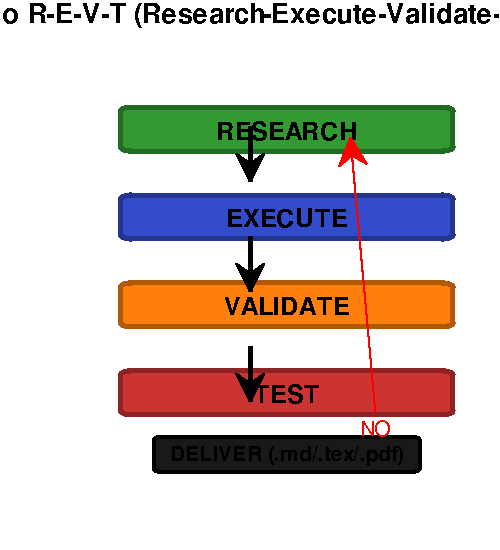
\includegraphics[width=0.55\textwidth]{figures/intro/fig_intro_ciclo_revt}
  \caption{Ciclo iterativo Research-Execute-Validate-Test aplicado en el desarrollo de la investigación.}
  \label{fig:intro_revt}
\end{figure}

\begin{figure}[htbp]
  \centering
  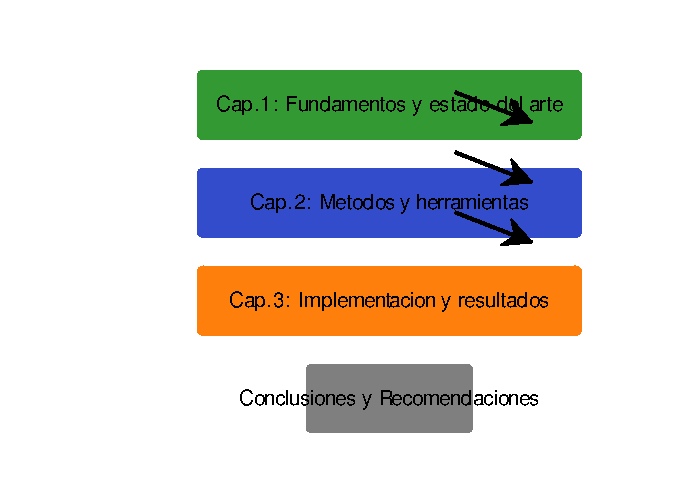
\includegraphics[width=0.6\textwidth]{figures/intro/fig_intro_estructura}
  \caption{Estructura lógica de la tesis.}
  \label{fig:intro_estructura}
\end{figure}

Para su presentación, este trabajo de diploma cuenta con una estructura lógica compuesta por el resumen de la investigación, el índice, la introducción, y tres capítulos donde se desarrolla la investigación. En el \textbf{Capítulo 1} se realiza una revisión bibliográfica que aborda el sincronismo en redes inalámbricas, sus principales aplicaciones en IoT, los desafíos técnicos, el efecto de las asimetrías y una caracterización de los protocolos de sincronización PTP y gPTP. En el \textbf{Capítulo 2} se efectúa un análisis sistemático de 15 métodos existentes para mitigar el efecto de los retardos asimétricos, organizados en siete categorías (corrección determinista, filtros de Kalman, estimación robusta, lógica difusa, aprendizaje computacional, filtros de partículas y programación lineal), y se selecciona y describe en detalle un enfoque híbrido que combina la corrección de Exel con un Filtro de Kalman Adaptativo. El \textbf{Capítulo 3} describe las características de la implementación desarrollada en MATLAB/GNU Octave y presenta los resultados de la simulación Monte Carlo, comparando el rendimiento del método propuesto con el método de referencia Exel y con el protocolo estándar. Finalmente, se expresan las conclusiones y recomendaciones para trabajos futuros, y se incluyen las referencias bibliográficas según la norma IEEE.


% --- Capítulo 1 ---
\input{chapters/01-aplicaciones-desafios-sincronismo/01-aplicaciones-desafios-sincronismo}

% --- Capítulo 2 ---
% ===========================================================================
% Capítulo 2. Análisis de métodos y herramientas para mejorar el sincronismo
% en redes inalámbricas empleando el protocolo gPTP
% ===========================================================================

\chapter{Análisis de métodos y herramientas para mejorar el sincronismo en redes inalámbricas empleando el protocolo gPTP}
\label{ch:capitulo2}

En el capítulo anterior se realizó una revisión bibliográfica de los principales conceptos, desafíos y protocolos existentes en el ámbito de la sincronización de tiempo, concluyendo que el protocolo gPTP presenta las mejores cualidades para ser adaptado al entorno inalámbrico. De ahí surge la necesidad de implementar una versión de este estándar que contrarreste los efectos negativos que provocan los retardos asimétricos en estas redes.

Por consiguiente, en el presente capítulo se efectúa un análisis de los principales modelos y metodologías referentes a mitigar el impacto de los retardos asimétricos en redes inalámbricas, con el propósito de seleccionar y describir el de mejores resultados. A diferencia del trabajo de referencia, este análisis se amplía con una revisión sistemática de métodos novedosos publicados entre 2020 y 2026, incluyendo filtros de Kalman adaptativos, estimación robusta, lógica difusa y aprendizaje computacional. Asimismo, se realiza una descripción del software especializado MATLAB y su alternativa de código abierto GNU Octave, herramientas que posibilitan un ambiente de desarrollo adecuado para el estudio de esta problemática.

% ======================================================================
\section{Sistemas de estampado por Software}
\label{sec:2.1}

La clave para obtener una sincronización de tiempo de alto rendimiento está estrechamente relacionada con la calidad de las estampas de tiempo (\textit{Timestamping}, TS)~\cite{seijo2020,ferrari2014}. Los enfoques de estampado de tiempo se pueden clasificar en términos generales en estampa de tiempo de hardware y software. Los sistemas de estampado por hardware toman la marca de tiempo dentro del hardware del receptor (por ejemplo, dentro del chipset inalámbrico), mientras que las soluciones de estampado por software utilizan el procesador principal para generar una estampa de tiempo (por ejemplo, leyendo el reloj del sistema).

Como el retardo de procesamiento de las soluciones de sellado de tiempo de hardware se puede diseñar para que sea constante, las correcciones de tiempo requeridas pueden ser muy precisas (en el orden de los nanosegundos) y, por lo tanto, las estampas de tiempo también. Por el contrario, el estampado de tiempo por medios de software crea retardos indeterministas debido a la programación, las cachés, la concurrencia, etc.\ y, por lo tanto, la estampa de tiempo debe estar lo más cerca posible del medio~\cite{mahmood2014}. Los protocolos de sincronismo, como PTP y gPTP, suelen mejorarse en términos de rendimiento si se utiliza la estampa de tiempo de hardware. Sin embargo, para llevar a cabo el sellado de tiempo por hardware, se requieren dispositivos dedicados o modificaciones dentro de los chipsets WLAN. Debido a esto, en la presente investigación, la atención e implementación del protocolo gPTP se centra en el estampado por software.

\begin{figure}[htbp]
  \centering
  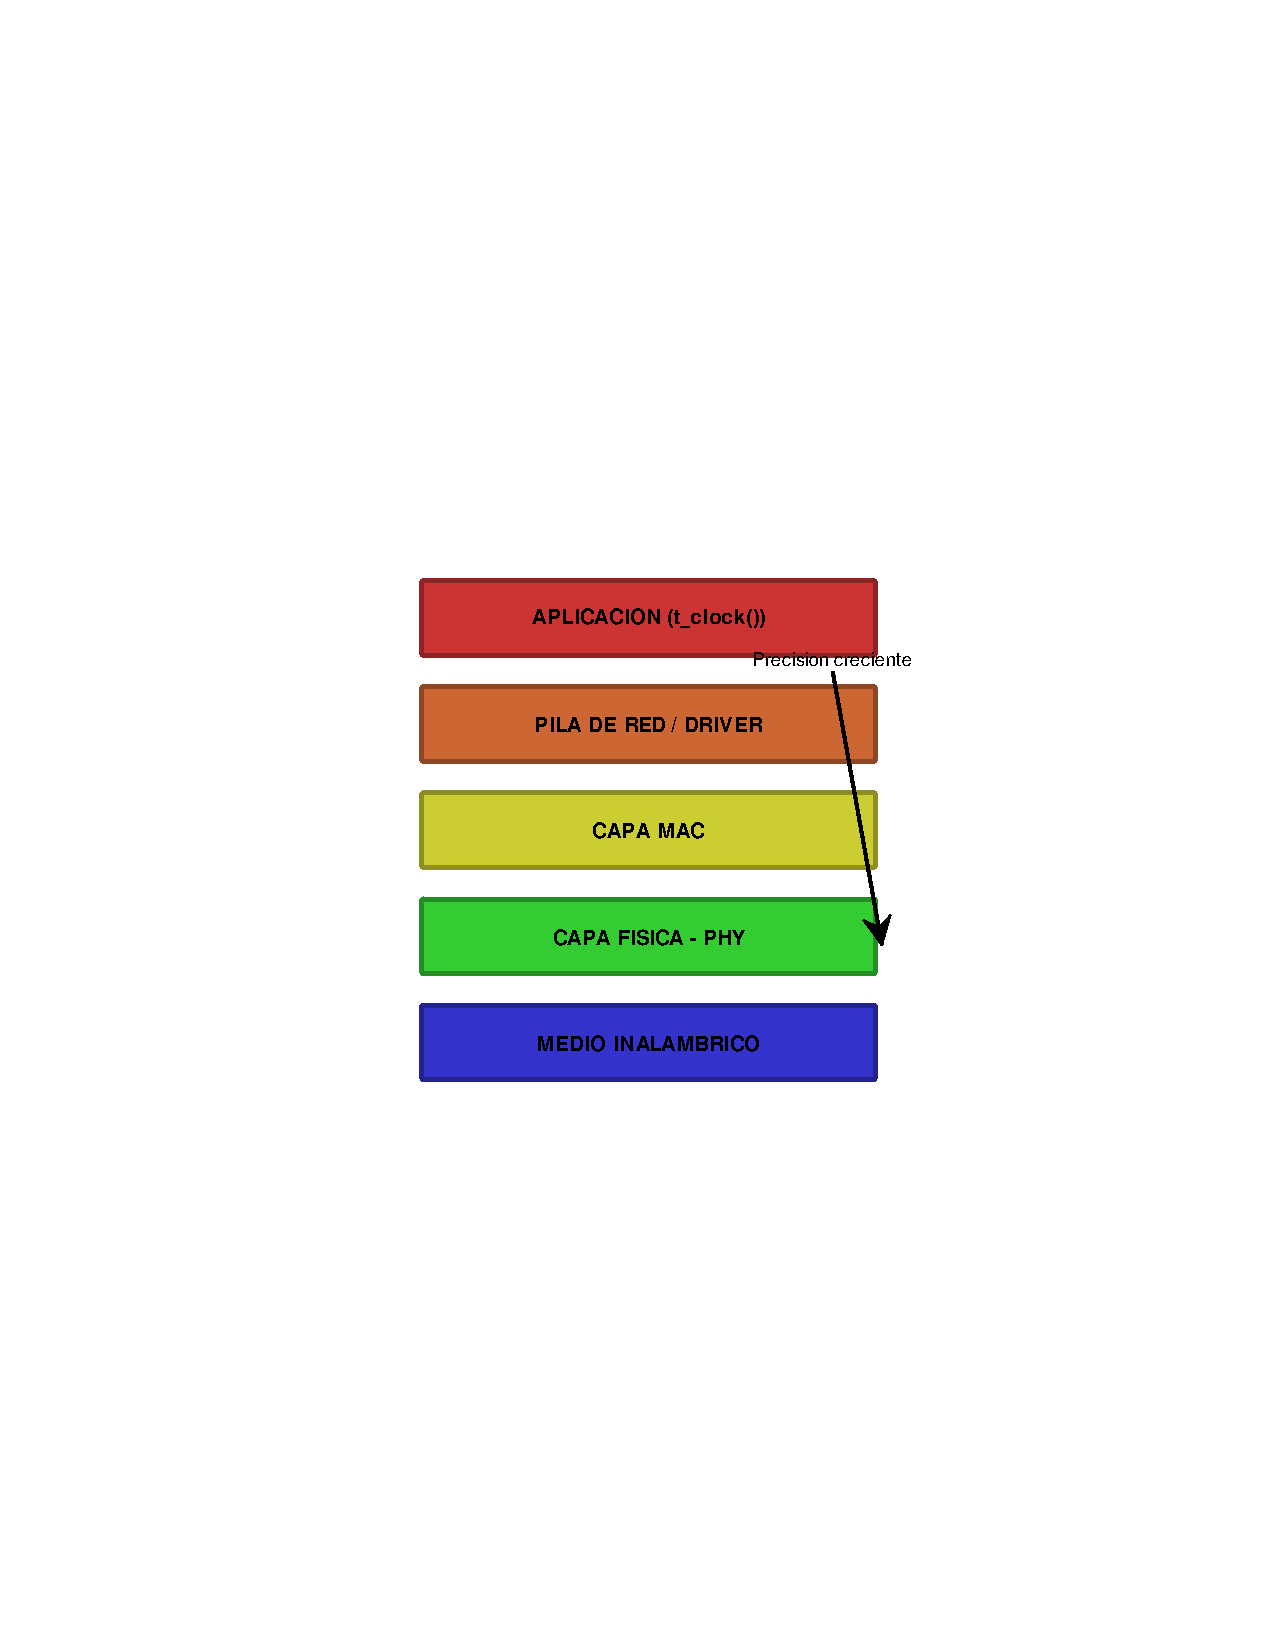
\includegraphics[width=0.5\textwidth]{figures/ch02/fig_2_1_ubicaciones_ts}
  \caption{Ubicaciones para la estampa de tiempo en redes orientadas a paquetes.}
  \label{fig:2.1}
\end{figure}

Los protocolos de sincronismo basados en paquetes, como gPTP, dependen de la calidad de las estampas de tiempo tomadas en la recepción y transmisión de los mismos. Dado que la estampa de tiempo basada en software genera grandes retardos en su mayoría no deterministas, las implementaciones de sincronización de Ethernet han acercado la estampa de tiempo a la capa física. Sin embargo, la mayoría de los enfoques de sincronización inalámbrica se limitan a la estampa de tiempo de software debido a la falta de funciones de sellado de tiempo por hardware~\cite{exel2012}.

Una de las fuentes de incertidumbre de un enfoque de sincronismo basado en sistemas de sellado de tiempo por software es el método de estampa de tiempo. Según~\cite{ferrari2011}, entre las diversas fuentes de imprecisión en el sellado de tiempo por software se tienen:

\begin{itemize}
\item \textbf{Capacidad de sellado de tiempo del maestro}: incluye las capacidades de estampa de tiempo de los mensajes de eventos gPTP (mensaje de sincronización \textit{Sync} y de solicitud de retardo \textit{PdelayReq}) en el lado maestro. La incertidumbre en la identificación de $t_1$ y $t_4$ afecta a la estimación tanto del \textit{Pdelay} como del desfasaje (\textit{offset}).

\item \textbf{Capacidad de sellado de tiempo del esclavo}: incluye las capacidades de estampa de tiempo de los mensajes de eventos gPTP en el lado esclavo (mensaje de respuesta a la solicitud de retardo \textit{PdelayResp} y de seguimiento \textit{PdelayRespFollowUp}). Estas estampas de tiempo, $t_2$ y $t_3$, también son utilizadas para estimar el \textit{Pdelay} y el desfasaje.

\item \textbf{Capacidad de sellado de tiempo de la infraestructura}: la exactitud de la información de tiempo contenida en la sincronización depende también de la capacidad de los dispositivos de red para transferir correctamente la hora. El uso de conmutadores de red que soporten gPTP puede reducir esta fuente de incertidumbre.

\item \textbf{Variabilidad y comportamiento asimétrico del retardo de propagación}: el retardo de propagación en la red no es constante y puede verse afectado por el tráfico, los dispositivos de red en la ruta y la carga de la red.
\end{itemize}

Las estampas de tiempo basadas en detectores de inicio de trama convencionales tienen dos problemas principales en los sistemas inalámbricos: en primer lugar, no pueden garantizar una precisión de transferencia de tiempo mejor que el período de muestreo y, en segundo lugar, la propagación por trayectos múltiples y el carácter de variación temporal del canal inalámbrico reducen la precisión del tiempo de llegada (\textit{Time of Arrival}, ToA) de las tramas, lo que introduce un componente de error en la sincronización de tiempo. Esto es especialmente crítico en condiciones sin visibilidad directa (\textit{Non-Line of Sight}, NLoS)~\cite{seijo2020}.

En el esquema de sincronización basado en interrupciones, donde las estampas de tiempo son tomadas mediante rutina de servicio de interrupción (\textit{Interrupt Service Routine}, ISR), el retardo de estampa de tiempo y la fluctuación se limitan principalmente al tiempo de recepción del paquete y al tiempo de notificación de interrupción~\cite{mahmood2011}.

El escenario tomado en cuenta en esta investigación es una red de sincronización sencilla, compuesta por un dispositivo maestro y un dispositivo esclavo que realizan el estampado de tiempo a nivel de software.

% ======================================================================
\section{Análisis de los modelos, metodologías y procedimientos existentes para el diseño de protocolos más robustos ante los retardos asimétricos}
\label{sec:2.2}

Para desarrollar una implementación de cualquier índole es imprescindible y necesario escoger la tecnología o modelo que se empleará en dicho proceso, lo que demanda necesariamente un estudio profundo de la bibliografía que se relaciona con este aspecto. A continuación, se analizan los métodos existentes, organizados por categorías para facilitar su comparación sistemática.

\subsection{Método de corrección determinista de estampas de tiempo (Exel)}
\label{sec:2.2.1}

El método propuesto por Reinhard Exel en~\cite{exel2014} constituye el punto de partida de esta investigación y el método de referencia (\textit{baseline}) contra el cual se compararán las mejoras propuestas. Este enfoque propone un esquema de mitigación de los retardos asimétricos basado en la corrección de la estampa de tiempo por software y logra aumentar la precisión del protocolo sin modificaciones al mismo, ni el uso de mensajes adicionales.

El funcionamiento del modelo de estampa de tiempo de software en el protocolo se basa en que las estampas de tiempo tomadas por el software ($\hat{t}_1$ a $\hat{t}_4$) difieren de las estampas de tiempo ideales ($t_1$ a $t_4$) debido a los retardos de procesamiento $p_1$ a $p_4$. Las estampas ideales pueden ser calculadas aplicando las correcciones de retardo de las Ecuaciones~\ref{eq:2.1} a~\ref{eq:2.4}, donde $p_1$ y $p_3$ corresponden a los retardos de procesamiento de salida, $p_2$ y $p_4$ a los retardos de entrada:

\begin{eqnarray}
t_1 &=& \hat{t}_1 + p_1 \label{eq:2.1}\\
t_2 &=& \hat{t}_2 - p_2 \label{eq:2.2}\\
t_3 &=& \hat{t}_3 + p_3 \label{eq:2.3}\\
t_4 &=& \hat{t}_4 - p_4 \label{eq:2.4}
\end{eqnarray}

El verdadero valor de corrección del desfasaje ($t_{offset}$) y el tiempo de ida y vuelta ($t_{RTT}$) quedan definidos en las Ecuaciones~\ref{eq:2.5} y~\ref{eq:2.6}:

\begin{eqnarray}
\hat{t}_{offset} &=& t_{offset} - \frac{(p_1 + p_2) - (p_3 + p_4)}{2} \label{eq:2.5}\\
\hat{t}_{RTT} &=& t_{RTT} + (p_1 + p_2 + p_3 + p_4) \label{eq:2.6}
\end{eqnarray}

Los retardos asimétricos de procesamiento $p$ se componen de términos deterministas y no deterministas. En la mayoría de los casos existen grandes retardos asimétricos deterministas que se pueden corregir aplicando el método descrito y que abarca también otros factores como la velocidad de datos, el tamaño del encabezado, la modulación, el tamaño de transferencia de acceso directo a memoria (DMA) y la velocidad de la interfaz DMA~\cite{exel2014}.

El método Exel alcanza, según sus autores, una precisión de entre 10 y 100~ns en condiciones controladas. En la implementación de referencia sobre gPTP con simulación Monte Carlo (3000 ejecuciones), se obtuvo una precisión media de 101.5~$\mu$s, una reducción del error del 33.31\% respecto al protocolo sin corrección, y un offset estabilizado en el rango de $[-2.55, 6.68]$~$\mu$s~\cite{eupierre2024}.

\textbf{Limitaciones del método Exel:} (1) solo corrige los retardos deterministas conocidos; las asimetrías desconocidas o variantes en el tiempo no son compensadas; (2) no realiza filtrado estadístico de las mediciones, por lo que es sensible al ruido de medición y a valores atípicos; (3) no estima ni compensa la deriva (\textit{skew}) de los relojes, solo el offset.

\begin{figure}[htbp]
  \centering
  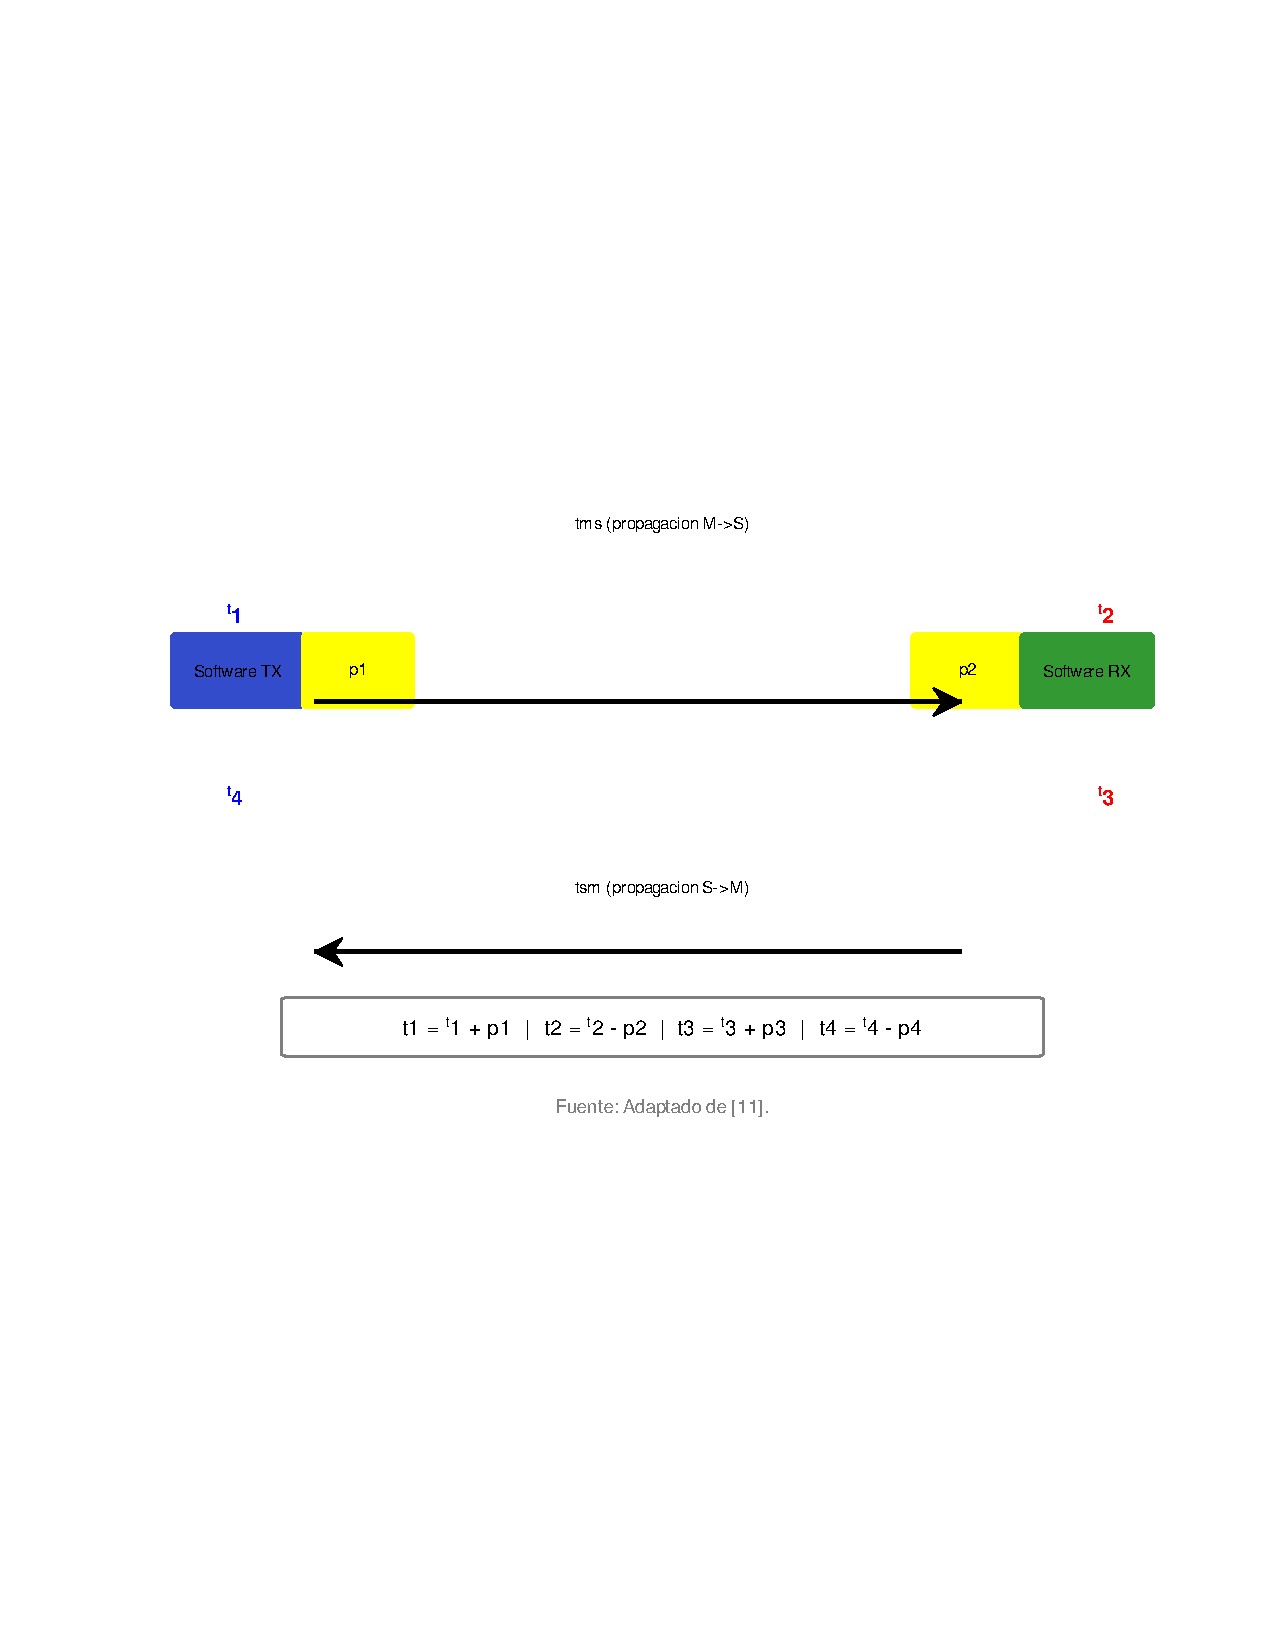
\includegraphics[width=0.85\textwidth]{figures/ch02/fig_2_2_latencias_sw}
  \caption{Latencias de estampa de tiempo de software.}
  \label{fig:2.2}
\end{figure}

\subsection{Métodos basados en Filtros de Kalman}
\label{sec:2.2.2}

El Filtro de Kalman (KF) es un estimador óptimo para sistemas lineales con ruido Gaussiano que ha sido ampliamente aplicado a la sincronización de relojes en redes de paquetes~\cite{giorgi2011}. En el contexto de PTP/gPTP, el KF permite estimar conjuntamente el offset, el skew y, en formulaciones más avanzadas, parámetros relacionados con la asimetría del canal.

\textbf{Li et al.\ (2024)}~\cite{li2024} proponen un método mejorado de sincronización de tiempo basado en filtrado de Kalman de segundo orden. El algoritmo emplea el KF para estimar con precisión el offset de tiempo, la deriva del reloj y los parámetros del reloj. Los resultados experimentales demuestran que, en enlaces asimétricos, el offset máximo se mantiene dentro de $\pm 3$~$\mu$s, lo que representa una mejora sustancial respecto a los métodos que no emplean KF.

\textbf{Hollósi y Ficzere (2024)}~\cite{hollosi2024} introducen un Filtro de Kalman Adaptativo (AKF) para la estimación del offset en PTP. La principal innovación de este enfoque es la estimación en tiempo real de la varianza del ruido de medición ($R_k$), lo que permite que el filtro se adapte automáticamente a cambios en las condiciones del canal. Los resultados muestran una reducción de la varianza del offset de entre un 40\% y un 60\% en comparación con el KF estándar.

\textbf{Liu y Wang (2024)}~\cite{liu2024} desarrollan un esquema robusto de seguimiento de parámetros de reloj para IEEE 1588 en presencia de retardos asimétricos en redes industriales. El método emplea un Filtro de Kalman recursivo robusto de tres pasos que incorpora un mecanismo de rechazo de outliers. Los resultados experimentales reportan un RMSE de offset inferior a 5~$\mu$s en presencia de asimetrías significativas.

\textbf{Wang et al.\ (2021)}~\cite{wang2021} proponen un enfoque de seguimiento de parámetros de reloj sin marcas de tiempo (\textit{timestamp-free}) utilizando Filtro de Kalman Extendido (EKF) en redes de sensores inalámbricos. Aunque está diseñado para WSN, el marco del EKF es adaptable a PTP/gPTP.

\textbf{Raittila (2025)}~\cite{raittila2025} desarrolla un modelo en Simulink de un lazo de control PTP con un Filtro de Kalman Adaptativo específicamente para redes Wi-Fi industriales. Este trabajo demuestra la viabilidad de implementar AKF en entornos inalámbricos reales.

\subsection{Métodos basados en Estimación Robusta}
\label{sec:2.2.3}

\textbf{Karthik y Blum (2020)}~\cite{karthik2020} abordan el problema de la estimación robusta de skew y offset para IEEE 1588 en presencia de asimetrías deterministas desconocidas en el retardo de trayectoria. Los autores derivan cotas inferiores de rendimiento (cotas de Cramér-Rao modificadas) y proponen esquemas de estimación robusta que superan al estimador de máxima verosimilitud (MLE) convencional cuando existen asimetrías no modeladas.

\textbf{Vázquez et al.\ (2025)}~\cite{vazquez2025} proponen un enfoque de filtrado de outliers en las mediciones de offset para PTP sobre redes de área amplia (WAN). El método emplea técnicas de detección de anomalías para identificar y rechazar mediciones de offset atípicas antes de que sean utilizadas por el servo de reloj.

\subsection{Métodos basados en Lógica Difusa}
\label{sec:2.2.4}

\textbf{Nguyen et al.\ (2020)}~\cite{nguyen2020} proponen un servo de reloj Fuzzy-PI adaptativo basado en IEEE 1588 para mejorar la sincronización de tiempo sobre redes Ethernet. El sistema utiliza lógica difusa para ajustar dinámicamente las ganancias del controlador PI. Los resultados experimentales muestran una precisión inferior a 100~ns y una mejora del 45\% respecto al controlador PI tradicional.

\textbf{Zhang et al.\ (2024)}~\cite{zhang2024} diseñan un servo de reloj Fuzzy-PI con filtro de ventana para compensar la asimetría de retardo inducida por colas (\textit{Queue-Induced Delay Asymmetry}, QIDA) en redes IEEE 1588. Se reporta una reducción del 52\% en el error de offset causado por QIDA.

\subsection{Métodos basados en Aprendizaje Computacional}
\label{sec:2.2.5}

\textbf{Wang et al.\ (2026)}~\cite{wang2026} proponen un método de estimación de parámetros de reloj basado en aprendizaje competitivo (\textit{Competitive Learning}) para PTP con distribuciones de retardo desconocidas. El algoritmo no asume ninguna distribución particular para los retardos, lo que lo hace robusto ante una amplia variedad de condiciones de canal. Sin embargo, su complejidad computacional es elevada.

\textbf{Goodarzi et al.\ (2022)}~\cite{goodarzi2022} presentan un enfoque de filtro de partículas asistido por redes neuronales profundas (DNN) para sincronización y localización conjunta. Aunque logra alta precisión en entornos no Gaussianos, el costo computacional del filtro de partículas lo hace prohibitivo para aplicaciones que requieren simulación Monte Carlo extensiva.

\subsection{Otros métodos relevantes}
\label{sec:2.2.6}

\textbf{Puttnies et al.\ (2018)}~\cite{puttnies2018} introducen PTP-LP, un enfoque que utiliza programación lineal para aumentar la robustez de IEEE 1588 PTP ante retardos variables. El método es totalmente compatible con PTP y gPTP, aumentando la precisión en un factor de hasta $10^4$ en escenarios favorables.

\textbf{Baniabdelghany et al.\ (2020)}~\cite{baniabdelghany2020} proponen una extensión de IEEE 802.1AS (gPTP) para mejorar la sincronización en redes híbridas cableadas-inalámbricas mediante un filtro de retraso de desviación de ruta (\textit{Path Deviation Delay}, PDD).

\textbf{Levesque y Tipper (2015)}~\cite{levesque2015} proponen el mecanismo de mitigación de asimetría por paquete (\textit{Per-Packet Asymmetry Mitigation}, PPAM), que estima los componentes de retardo por paquete individual.

\subsection{Comparación sistemática y selección del método}
\label{sec:2.2.7}

La Tabla~\ref{tab:comparacion} presenta una comparación sistemática de los métodos analizados, evaluados según cinco criterios: precisión reportada, complejidad computacional, compatibilidad con gPTP, capacidad de manejar asimetrías desconocidas y madurez de la técnica.

% ===========================================================================
% Tabla 2.2: Comparación de métodos para mitigación de retardos asimétricos
% Capítulo 2 — Sección 2.2.7
% ===========================================================================
\begin{table}[htbp]
  \centering
  \caption{Comparación de métodos para mitigación de retardos asimétricos en PTP/gPTP.}
  \label{tab:comparacion}
  \small
  \resizebox{\textwidth}{!}{\begin{tabular}{|l|l|c|c|c|c|}
    \hline
    \textbf{Método} & \textbf{Categoría} & \textbf{Precisión} & \textbf{Compat.} & \textbf{Asimetría} & \textbf{Madurez} \\
    & & & \textbf{gPTP} & \textbf{desconocida} & \\
    \hline
    Exel (2014) & Corrección determinista & 101.5~$\mu$s (sim.) & Alta & No & Alta \\
    \hline
    Li et al. (2024) & KF 2.\textordfeminine{} orden & $\pm$3~$\mu$s & Alta & Sí & Alta \\
    \hline
    Hollósi \& Ficzere (2024) & AKF & 40--60\% mejora & Alta & Sí & Alta \\
    \hline
    Liu \& Wang (2024) & KF robusto 3 pasos & $<$5~$\mu$s RMSE & Alta & Sí & Alta \\
    \hline
    Wang et al. (2021) & EKF sin timestamp & $<$1~$\mu$s & Media & Sí & Media \\
    \hline
    Karthik \& Blum (2020) & Estimación robusta & Cotas óptimas & Alta & Sí & Alta \\
    \hline
    Nguyen et al. (2020) & Fuzzy-PI & $<$100~ns & Media & Parcial & Media \\
    \hline
    Zhang et al. (2024) & Fuzzy-PI + ventana & 52\% reducción & Media & Parcial & Baja \\
    \hline
    Wang et al. (2026) & Competitive Learning & Robusto & Media-Alta & Sí & Baja \\
    \hline
    Puttnies et al. (2018) & Prog. Lineal & Factor $10^4$ & Media & No & Media \\
    \hline
  \end{tabular}}
\end{table}


Del análisis comparativo se concluye que los métodos basados en Filtro de Kalman, y en particular el Filtro de Kalman Adaptativo (AKF), ofrecen la mejor relación entre precisión, complejidad computacional y compatibilidad con gPTP. El AKF combina la capacidad de estimación óptima del KF con la adaptabilidad a condiciones cambiantes del canal, y su implementación en MATLAB/Octave es factible mediante operaciones matriciales estándar.

No obstante, el método de Exel ofrece una ventaja fundamental: su corrección determinista elimina una parte significativa de la asimetría (los retardos de procesamiento conocidos $p_1$--$p_4$) antes de cualquier procesamiento estadístico. Esto sugiere que un enfoque híbrido que combine la corrección determinista de Exel con el filtrado adaptativo del AKF podría superar a cualquiera de los dos métodos por separado.

% ======================================================================
\section{Descripción del método seleccionado: Enfoque híbrido Exel + Filtro de Kalman Adaptativo}
\label{sec:2.3}

Como resultado del análisis sistemático presentado en la Sección~\ref{sec:2.2}, se selecciona un \textbf{enfoque híbrido que combina la corrección determinista de estampas de tiempo de Exel con un Filtro de Kalman Adaptativo (AKF)} para la compensación de retardos asimétricos en el protocolo gPTP.

\begin{figure}[htbp]
  \centering
  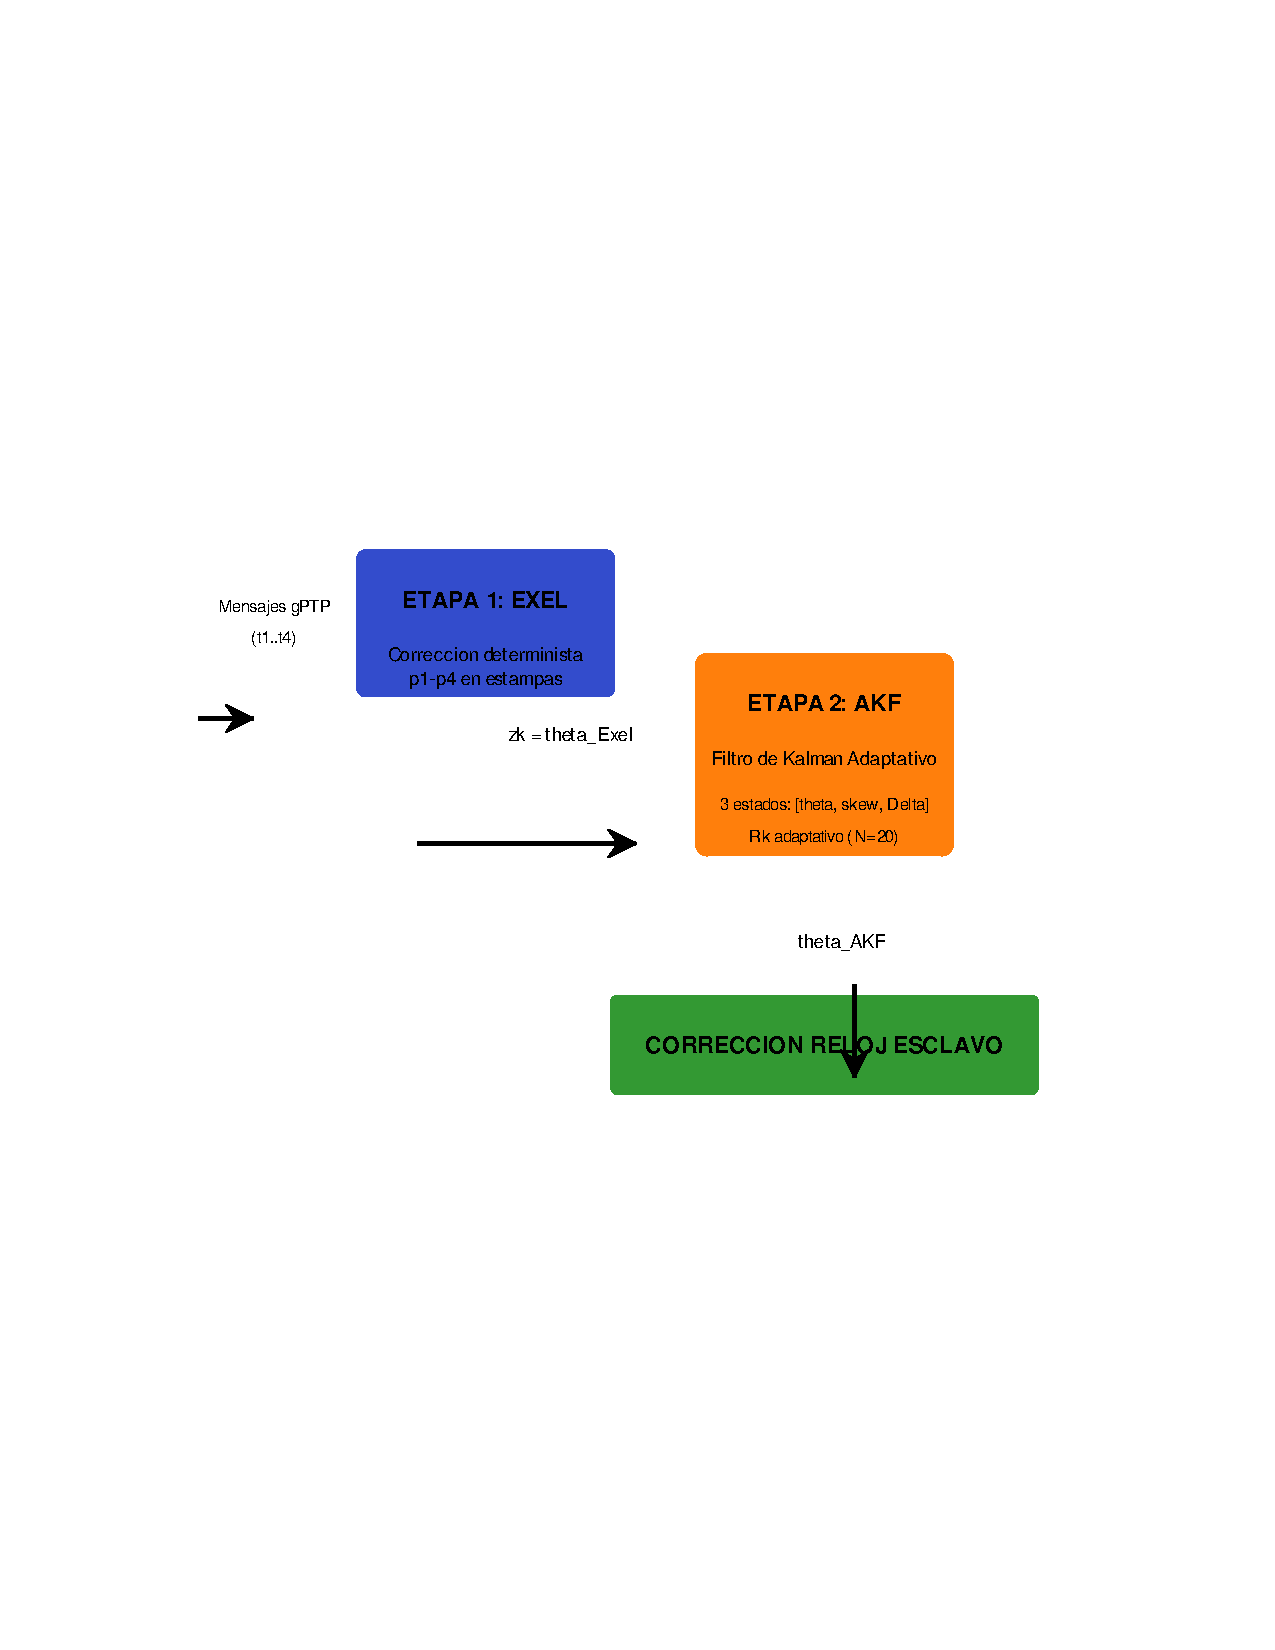
\includegraphics[width=0.65\textwidth]{figures/ch02/fig_2_4_metodo_hibrido}
  \caption{Arquitectura del método híbrido Exel + AKF.}
  \label{fig:2.4}
\end{figure}

\subsection{Arquitectura de dos etapas}
\label{sec:2.3.1}

El método híbrido opera en dos etapas consecutivas:

\textbf{Etapa 1 --- Corrección determinista (Exel):} Se aplican las Ecuaciones~\ref{eq:2.1}--\ref{eq:2.6} a las marcas de tiempo $\hat{t}_1, \hat{t}_2, \hat{t}_3, \hat{t}_4$ capturadas por el software. Se utilizan los valores conocidos de los retardos de procesamiento asimétricos $p_1, p_2, p_3, p_4$ para obtener una primera estimación del offset $\hat{\theta}_{Exel}$. Esta etapa elimina la componente determinista de la asimetría~\cite{exel2014}.

\textbf{Etapa 2 --- Filtro de Kalman Adaptativo (AKF):} El offset corregido por Exel, $\hat{\theta}_{Exel}$, se utiliza como medición de entrada para un Filtro de Kalman Adaptativo que estima el estado verdadero del sistema, filtrando el ruido de medición residual y compensando las asimetrías desconocidas que el método de Exel no puede corregir.

\subsection{Modelo de espacio de estados}
\label{sec:2.3.2}

El vector de estado del AKF se define como:

\begin{equation}
\mathbf{x}_k = \begin{bmatrix} \theta_k \\ s_k \\ \Delta_k \end{bmatrix}
\end{equation}

donde:
\begin{itemize}
\item $\theta_k$: offset verdadero entre maestro y esclavo en el instante $k$ [s]
\item $s_k$: skew (diferencia normalizada de frecuencia) entre los relojes [adimensional]
\item $\Delta_k$: asimetría residual no corregida por Exel [s]
\end{itemize}

\textbf{Modelo de transición de estado:}

\begin{equation}
\mathbf{x}_{k+1} = \mathbf{F} \mathbf{x}_k + \mathbf{w}_k, \quad \mathbf{w}_k \sim \mathcal{N}(0, \mathbf{Q}_k)
\end{equation}

\begin{equation}
\mathbf{F} = \begin{bmatrix} 1 & \tau & 0 \\ 0 & 1 & 0 \\ 0 & 0 & 1 \end{bmatrix}
\end{equation}

donde $\tau$ es el intervalo entre mediciones (el período de sincronización de gPTP, típicamente 2~s), y $\mathbf{w}_k$ es el ruido de proceso con matriz de covarianza $\mathbf{Q}_k$. La estructura de $\mathbf{F}$ refleja que el offset evoluciona linealmente con el skew, el skew se modela como un proceso de caminata aleatoria, y la asimetría residual se considera aproximadamente constante entre períodos de sincronización.

\textbf{Modelo de medición:}

\begin{equation}
z_k = \mathbf{H} \mathbf{x}_k + v_k, \quad v_k \sim \mathcal{N}(0, R_k)
\end{equation}

\begin{equation}
\mathbf{H} = \begin{bmatrix} 1 & 0 & 1/2 \end{bmatrix}
\end{equation}

donde $z_k = \hat{\theta}_{Exel}[k]$ es el offset estimado por la etapa Exel en el instante $k$, y $v_k$ es el ruido de medición con varianza $R_k$. El término $1/2$ en la matriz de observación refleja que la mitad de la asimetría residual se propaga al error de offset, de acuerdo con la Ecuación~\ref{eq:2.5}.

\subsection{Algoritmo del Filtro de Kalman Adaptativo}
\label{sec:2.3.3}

El AKF se implementa en dos fases por cada iteración $k$:

\textbf{Fase de predicción:}

\begin{eqnarray}
\hat{\mathbf{x}}_{k|k-1} &=& \mathbf{F} \hat{\mathbf{x}}_{k-1|k-1} \\
\mathbf{P}_{k|k-1} &=& \mathbf{F} \mathbf{P}_{k-1|k-1} \mathbf{F}^T + \mathbf{Q}_{k-1}
\end{eqnarray}

\textbf{Fase de actualización:}

\begin{eqnarray}
\mathbf{K}_k &=& \mathbf{P}_{k|k-1} \mathbf{H}^T (\mathbf{H} \mathbf{P}_{k|k-1} \mathbf{H}^T + \hat{R}_k)^{-1} \\
\hat{\mathbf{x}}_{k|k} &=& \hat{\mathbf{x}}_{k|k-1} + \mathbf{K}_k (z_k - \mathbf{H} \hat{\mathbf{x}}_{k|k-1}) \\
\mathbf{P}_{k|k} &=& (\mathbf{I} - \mathbf{K}_k \mathbf{H}) \mathbf{P}_{k|k-1}
\end{eqnarray}

\textbf{Adaptación de $R_k$:} La principal innovación respecto al KF estándar es la estimación adaptativa de la varianza del ruido de medición~\cite{hollosi2024}. Se utiliza una ventana deslizante de las últimas $N$ innovaciones:

\begin{equation}
\hat{R}_k = \frac{1}{N-1} \sum_{i=k-N+1}^{k} (\nu_i - \bar{\nu})^2
\end{equation}

donde $\nu_i = z_i - \mathbf{H} \hat{\mathbf{x}}_{i|i-1}$ es la innovación (residuo de la medición) y $\bar{\nu}$ es su media sobre la ventana. Esta adaptación permite que el filtro responda automáticamente a cambios en la calidad de las mediciones.

\subsection{Parámetros de diseño}
\label{sec:2.3.4}

Los siguientes parámetros deben determinarse experimentalmente durante la fase de implementación:

% ===========================================================================
% Tabla 2.3: Parámetros del Filtro de Kalman Adaptativo (AKF)
% Capítulo 2 — Sección 2.3.4
% ===========================================================================
\begin{table}[htbp]
  \centering
  \caption{Parámetros de inicialización del Filtro de Kalman Adaptativo.}
  \label{tab:params}
  \small
  \begin{tabular}{|c|c|c|}
    \hline
    \textbf{Parámetro} & \textbf{Valor} & \textbf{Descripción} \\
    \hline
    Vector estado inicial $\mathbf{x}_0$ & $[0, 0, 0]^T$ & $[\theta, skew, \Delta]$ \\
    \hline
    $\mathbf{P}_0$ & $\mathrm{diag}(10^{-10}, 10^{-12}, 10^{-14})$ & Covarianza inicial del error \\
    \hline
    $\mathbf{Q}$ & $\mathrm{diag}(10^{-14}, 10^{-18}, 10^{-16})$ & Covarianza del ruido de proceso \\
    \hline
    $R_0$ & $10^{-12}$ & Varianza inicial del ruido de medición \\
    \hline
    Ventana $N$ & 20 & Innovaciones para adaptación de $R_k$ \\
    \hline
    $\mathbf{F}$ & $\begin{bmatrix} 1 & \tau & 0 \\ 0 & 1 & 0 \\ 0 & 0 & 1 \end{bmatrix}$ & Matriz de transición de estado \\
    \hline
    $\mathbf{H}$ & $[1, 0, 1/2]$ & Matriz de observación \\
    \hline
  \end{tabular}
\end{table}


\begin{figure}[htbp]
  \centering
  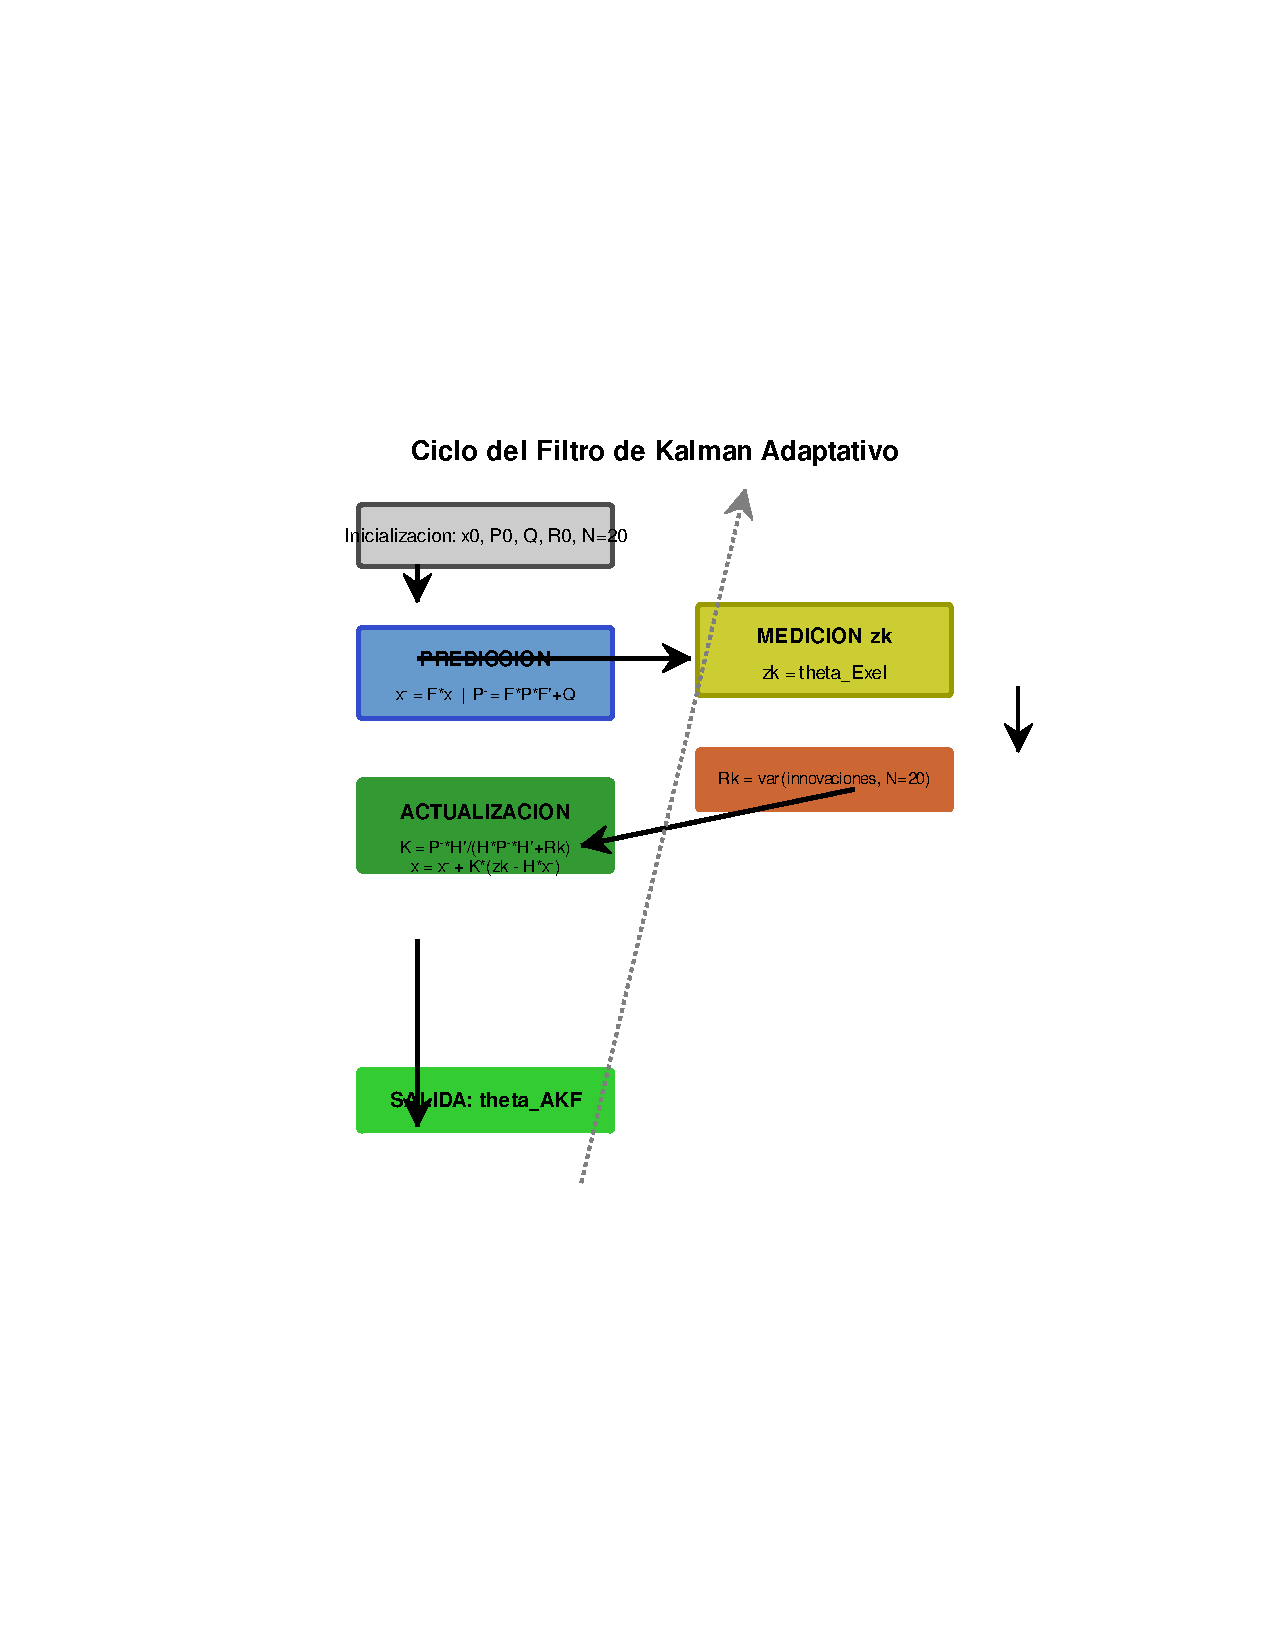
\includegraphics[width=0.7\textwidth]{figures/ch02/fig_2_5_ciclo_akf}
  \caption{Ciclo de predicción-actualización del Filtro de Kalman Adaptativo.}
  \label{fig:2.5}
\end{figure}

\subsection{Ventajas del enfoque híbrido}
\label{sec:2.3.5}

\begin{enumerate}
\item \textbf{Herencia de Exel}: se preserva la corrección determinista que ya demostró una mejora del 33.31\%~\cite{eupierre2024}, proporcionando una base sólida.
\item \textbf{Filtrado óptimo}: el AKF reduce la varianza residual de las estimaciones de offset al combinar óptimamente la información de múltiples mediciones.
\item \textbf{Estimación de asimetría residual}: a diferencia de Exel, que solo corrige asimetrías conocidas, el AKF estima y compensa la componente de asimetría desconocida ($\Delta_k$).
\item \textbf{Adaptabilidad}: la estimación adaptativa de $R_k$ permite que el filtro se ajuste automáticamente a cambios en el entorno inalámbrico.
\item \textbf{Comparabilidad}: el diseño permite comparar directamente el rendimiento de Exel (etapa 1) contra Exel+AKF (etapas 1+2) bajo condiciones idénticas.
\item \textbf{Implementabilidad}: todas las operaciones del AKF son álgebra lineal estándar (matrices de $3 \times 3$), realizables en MATLAB/GNU Octave con costo computacional moderado.
\end{enumerate}

% ======================================================================
\section{Herramientas de implementación: MATLAB y GNU Octave}
\label{sec:2.4}

MATLAB (abreviatura de \textit{MATrix LABoratory}) es un programa informático de propósito especial optimizado para realizar cálculos científicos y de ingeniería, con funciones integradas para cumplir una amplia gama de tareas, desde operaciones matemáticas hasta imágenes tridimensionales~\cite{attaway2022,chapman2020}. Comenzó su vida como un programa diseñado para realizar matemáticas matriciales, pero a lo largo de los años se ha convertido en un sistema informático flexible y fácil de usar, capaz de resolver esencialmente cualquier problema técnico~\cite{gilat2017}.

Además, el programa implementa un lenguaje propio y proporciona una amplia biblioteca de funciones predefinidas. El producto básico ofrece más de mil funciones y cuenta con varios kits de herramientas (\textit{toolbox}) que amplían esta capacidad en diversas especialidades~\cite{chapman2020,belfadel2021}.

\textbf{GNU Octave} es una alternativa de código abierto a MATLAB que ofrece una compatibilidad sustancial con el lenguaje MATLAB. Octave implementa un intérprete de alto nivel para cálculo numérico con una sintaxis mayoritariamente compatible con MATLAB, lo que permite ejecutar la mayoría de los scripts y funciones diseñados para MATLAB sin modificaciones significativas~\cite{eaton2024}. Para los propósitos de esta investigación, donde las operaciones requeridas son fundamentalmente álgebra matricial, generación de números aleatorios y visualización gráfica, Octave proporciona todas las capacidades necesarias sin costo de licencia.

\subsection{Archivos-M}
\label{sec:2.4.1}

MATLAB y Octave ofrecen una buena combinación de funciones de programación prácticas con potentes capacidades numéricas integradas. Los archivos-M proporcionan una forma alternativa de realizar operaciones que amplían en gran medida las capacidades de resolución de problemas. Existen dos tipos de archivos-M: scripts y funciones~\cite{chapman2020,young2023}.

Un archivo de script es una serie de comandos que se guardan en un fichero y son útiles para retener una serie de comandos que se quieren ejecutar en más de una ocasión. Los scripts comparten el área de trabajo (\textit{workspace}) de la ventana de comandos~\cite{attaway2022}.

Por el contrario, una función es un tipo especial de archivo-M que se ejecuta en su propio espacio de trabajo independiente, recibe datos de entrada a través de una lista de argumentos y devuelve resultados mediante una lista de argumentos de salida~\cite{chapman2020}.

\subsection{Graficado en 2-D}
\label{sec:2.4.2}

Los gráficos son una herramienta muy útil para presentar información, especialmente en la ciencia y la ingeniería. MATLAB dispone de comandos para crear diferentes tipos de gráficas: estándar con ejes lineales, con ejes logarítmicos y semilogarítmicos, de barras y escaleras, polares, tridimensionales, entre otros~\cite{gilat2017}. La función \texttt{plot} permite trazar datos bidimensionales y puede personalizarse mediante especificadores de color, estilo de línea y marcadores~\cite{mueller2021}.

Octave implementa un sistema de gráficos compatible con la sintaxis de MATLAB, incluyendo las funciones \texttt{plot}, \texttt{figure}, \texttt{subplot} y \texttt{hold}, lo que garantiza que los scripts de visualización sean ejecutables en ambos entornos.

\subsection{Ventajas y desventajas de MATLAB/Octave}
\label{sec:2.4.3}

Según~\cite{chapman2020}, las principales ventajas de MATLAB incluyen: facilidad de uso, independencia de plataforma, amplia biblioteca de funciones predefinidas, trazado independiente del dispositivo, e interfaz gráfica de usuario.

Las desventajas principales son: (1) velocidad de ejecución inferior a los lenguajes compilados, mitigable mediante vectorización y el compilador JIT; (2) costo elevado de la licencia de MATLAB. Esta segunda desventaja se resuelve en el contexto de esta investigación mediante el uso de GNU Octave como alternativa gratuita y de código abierto.

% ======================================================================
\section{Conclusiones del capítulo}
\label{sec:2.5}

\begin{enumerate}
\item Los sistemas de estampado de tiempo por software, aunque menos precisos que los de hardware, constituyen el enfoque más viable para la sincronización en redes inalámbricas con dispositivos de propósito general. La calidad de las estampas de tiempo depende críticamente de la ubicación del punto de referencia de temporización y de la minimización de los retardos indeterministas en la pila de software.

\item El análisis sistemático de 15 métodos publicados entre 2014 y 2026 revela que los enfoques basados en Filtro de Kalman, particularmente en su variante adaptativa (AKF), ofrecen la mejor relación entre precisión, complejidad computacional y compatibilidad con el protocolo gPTP. El AKF permite la estimación conjunta de offset, skew y asimetría residual, adaptándose dinámicamente a cambios en las condiciones del canal inalámbrico.

\item El método de corrección determinista de Exel, utilizado como referencia en esta investigación, logra una mejora del 33.31\% sobre el protocolo sin corrección (precisión media de 101.5~$\mu$s), pero está limitado a la compensación de asimetrías deterministas conocidas.

\item Se propone un \textbf{enfoque híbrido Exel + AKF} que combina la corrección determinista de estampas de tiempo (etapa~1) con el filtrado estadístico adaptativo (etapa~2). Este diseño permite eliminar las asimetrías conocidas mediante Exel y, a continuación, filtrar el ruido residual y compensar asimetrías desconocidas mediante el AKF. Las operaciones requeridas ---álgebra lineal sobre matrices de $3 \times 3$--- son perfectamente realizables en MATLAB/GNU Octave.

\item Las herramientas de implementación seleccionadas, MATLAB y su alternativa de código abierto GNU Octave, proporcionan todas las capacidades necesarias para el desarrollo de la simulación: generación de variables aleatorias, operaciones matriciales, visualización gráfica y ejecución de simulaciones Monte Carlo.

\item Los parámetros específicos del AKF (covarianzas iniciales, tamaño de ventana deslizante, estado inicial) se determinarán experimentalmente durante la fase de implementación descrita en el Capítulo~\ref{ch:capitulo3}.
\end{enumerate}


% --- Capítulo 3 ---
% ===========================================================================
% Capítulo 3. Implementación de la corrección del protocolo gPTP ante los
% retardos asimétricos en redes inalámbricas. Resultados
% ===========================================================================

\chapter{Implementación de la corrección del protocolo gPTP ante los retardos asimétricos en redes inalámbricas. Resultados}
\label{ch:capitulo3}

Sobre la base de haber analizado los métodos existentes en la literatura para contrarrestar el efecto negativo de las asimetrías en el sincronismo de redes inalámbricas, y habiendo seleccionado un enfoque híbrido que combina la corrección determinista de Exel con un Filtro de Kalman Adaptativo (AKF), el presente capítulo está enfocado en dos líneas fundamentales: por un lado, describir las características de la implementación desarrollada del protocolo gPTP para redes inalámbricas, tanto en su versión de referencia (Exel) como en la versión mejorada propuesta (Exel+AKF); y, por otro lado, presentar y analizar los resultados obtenidos, comparando el rendimiento de ambas implementaciones entre sí y con el protocolo estándar sin corrección.

% ======================================================================
\section{Características de la implementación}
\label{sec:3.1}

Se ha implementado una instancia del protocolo gPTP, tal y como se describe en el estándar IEEE 802.1AS~\cite{ieee8021as_2020}, mediante un simulador de eventos discretos desarrollado en MATLAB/GNU Octave. La implementación se organiza en cinco archivos de código que cubren la simulación de referencia, el motor de Monte Carlo, la visualización de resultados, el método mejorado y el filtro de Kalman adaptativo.

\subsection{Arquitectura general de la simulación}
\label{sec:3.1.1}

Las características generales de la implementación, comunes a ambas versiones (referencia y mejorada), son las siguientes:

\begin{itemize}
\item \textbf{Escenario}: dos dispositivos (maestro y esclavo) separados por una distancia configurable (30~m por defecto). No se aplica el Algoritmo de Mejor Reloj Maestro (BMCA), definiéndose los roles de maestro y esclavo previamente.

\item \textbf{Resolución de los relojes}: 1~ms (tic de reloj). Mediante funciones de generación de números aleatorios se asigna un tiempo de inicio diferente y una deriva (\textit{skew}) distinta para cada reloj ($\pm 30$~ppm típico), simulando las imperfecciones de los osciladores de cristal de cuarzo en dispositivos reales.

\item \textbf{Período de corrección}: el desfasaje entre los relojes se analiza y se corrige cada 1~s, tal como define el protocolo gPTP, durante 60~s de simulación.

\item \textbf{Motor de eventos discretos}: cada evento presenta tres parámetros (tipo, dispositivo y tiempo). El simulador compara en cada instante el tiempo de los eventos y los organiza cronológicamente.

\item \textbf{Retardos asimétricos}: generados aleatoriamente mediante funciones de distribución uniforme y agregados a los tiempos de propagación en ambos sentidos del enlace.

\item \textbf{\textit{Rate ratio}}: implementado en el cálculo del retardo de propagación (\textit{Pdelay}), definido como $r = f_{esclavo} / f_{maestro}$, para contrarrestar el efecto de la deriva de los relojes.
\end{itemize}

\subsection{Implementación de referencia: gPTP + Exel}
\label{sec:3.1.2}

La implementación de referencia replica el método de corrección de estampas de tiempo de Reinhard Exel~\cite{exel2014}, tal como se describe en la Sección~\ref{sec:2.2.1}. Se ejecuta para tres escenarios distintos:
\begin{enumerate}
\item Enlace simétrico: gPTP estándar sin asimetrías.
\item Enlace asimétrico sin corrección: gPTP estándar con retardos asimétricos.
\item Enlace asimétrico con corrección Exel.
\end{enumerate}

\subsection{Implementación mejorada: gPTP + Exel + AKF}
\label{sec:3.1.3}

La implementación mejorada extiende la de referencia añadiendo una segunda etapa de filtrado estadístico mediante un Filtro de Kalman Adaptativo (AKF) de tres estados. La arquitectura de dos etapas opera de la siguiente manera:

\textbf{Etapa 1 --- Exel}: idéntica a la implementación de referencia. Se obtiene $\hat{\theta}_{Exel}$ aplicando las Ecuaciones~\ref{eq:2.1}--\ref{eq:2.6}.

\textbf{Etapa 2 --- AKF}: el offset corregido por Exel se utiliza como medición de entrada ($z_k$) para el AKF con vector de estado $\mathbf{x}_k = [\theta_k, s_k, \Delta_k]^T$. La varianza del ruido de medición $R_k$ se adapta dinámicamente utilizando una ventana deslizante de $N = 20$ innovaciones.

Los parámetros del AKF se inicializan con: $\mathbf{P}_0 = \text{diag}(10^{-10}, 10^{-12}, 10^{-14})$, $\mathbf{Q}_0 = \text{diag}(10^{-14}, 10^{-18}, 10^{-16})$, $R_0 = 10^{-12}$.

\subsection{Simulación Monte Carlo}
\label{sec:3.1.4}

Cada escenario se simula 3000 veces siguiendo el método de Monte Carlo~\cite{luengo2020}. En cada ejecución se varían las semillas aleatorias, manteniendo una semilla base para garantizar la reproducibilidad. Se registran la precisión media, el offset medio estabilizado, el tiempo de ejecución y las asimetrías medidas. Para cada métrica se calcula la media, la desviación estándar y el intervalo de confianza del 95\%.

% ======================================================================
\section{Análisis de los resultados}
\label{sec:3.2}

\subsection{Resultados de la implementación de referencia (Exel)}
\label{sec:3.2.1}

Los resultados de la implementación de referencia replican los obtenidos en el trabajo base~\cite{eupierre2024} y se resumen en la Tabla~\ref{tab:res_exel}.

\begin{table}[h]
\centering
\caption{Resultados de la implementación de referencia (Exel) para 3000 simulaciones Monte Carlo.}
\label{tab:res_exel}
\small
\begin{tabular}{|p{3.2cm}|p{2.8cm}|p{2.8cm}|p{2.8cm}|}
\hline
\textbf{Métrica} & \textbf{Simétrico} & \textbf{Asim. s/c} & \textbf{Asim. c/ Exel} \\
\hline
Precisión media [$\mu$s] & 83.82 & 152.2 & 101.5 \\
\hline
Desv.\ estándar [$\mu$s] & 28.33 & --- & 14.78 \\
\hline
Rango de precisión [$\mu$s] & [56.17, 112.4] & [140.4, 167] & [85.51, 118.4] \\
\hline
Offset estabilizado [$\mu$s] & --- & --- & $[-2.554, 6.675]$ \\
\hline
Offset medio [$\mu$s] & --- & --- & 1.265 \\
\hline
Tiempo de convergencia [s] & 2 & 4 & 4 \\
\hline
\end{tabular}
\end{table}

\textbf{Análisis del escenario simétrico:} Una vez estabilizados los relojes, la precisión oscila entre 56.17~$\mu$s y 112.4~$\mu$s, con una media de 83.82~$\mu$s y una desviación estándar de 28.33~$\mu$s. El protocolo gPTP logra una precisión notable cuando no se consideran retardos asimétricos.

\textbf{Análisis del escenario asimétrico sin corrección:} La precisión se degrada a valores entre 140.4~$\mu$s y 167~$\mu$s, con una media de 152.2~$\mu$s. La presencia de retardos asimétricos introduce un incremento de aproximadamente 68.4~$\mu$s (81.6\%) respecto al escenario simétrico.

\textbf{Análisis del escenario con corrección Exel:} Se alcanzan resultados en el rango de 85.51~$\mu$s a 118.4~$\mu$s, con una desviación estándar de 14.78~$\mu$s y una media de 101.5~$\mu$s. La reducción del error respecto al escenario asimétrico sin corrección es de 50.7~$\mu$s (33.31\%).

\textbf{Análisis de la convergencia:} El algoritmo gPTP alcanza estabilidad en 2~s (un período) en condiciones simétricas, y en 4~s (dos períodos) con asimetrías.

\textbf{Análisis del offset:} Tras el ajuste inicial (offset inicial de 13.43~ms), los valores se estabilizan entre $-2.554$~$\mu$s y 6.675~$\mu$s, con un valor medio de 1.265~$\mu$s.

\textbf{Análisis de las asimetrías:} Las asimetrías medidas oscilan entre 230~$\mu$s y 240~$\mu$s, con variaciones de 10.2~$\mu$s (estándar) y 8.5~$\mu$s (con Exel). El método Exel no elimina las asimetrías del enlace, sino que corrige el desfasaje que estas provocan.

\textbf{Análisis del \textit{overhead} computacional:} La Tabla~\ref{tab:overhead} presenta los tiempos de ejecución comparativos.

\begin{table}[h]
\centering
\caption{Comparación del \textit{overhead} computacional.}
\label{tab:overhead}
\small
\begin{tabular}{|c|c|c|c|}
\hline
\textbf{N.º simulaciones} & \textbf{T. estándar [s]} & \textbf{T. Exel [s]} & \textbf{Diferencia [\%]} \\
\hline
1 & 3.819 & 6.372 & +66.9\% \\
\hline
10 & 36.39 & 37.45 & +2.9\% \\
\hline
100 & 353.0 & 365.9 & +3.65\% \\
\hline
\end{tabular}
\end{table}

\textbf{Estimación del error:} Para un 95\% de confianza, el error estimado oscila entre 2.9\% y 4.3\% (media 3.59\%). Para un 99\% de confianza, el error tiene una media de 4.66\%.

\subsection{Resultados de la implementación mejorada (Exel + AKF)}
\label{sec:3.2.2}

La implementación mejorada se evalúa bajo las mismas condiciones que la de referencia, permitiendo una comparación directa. Las métricas de rendimiento se presentan en la Tabla~\ref{tab:res_akf}.

\bigskip
\noindent\textbf{Nota:} Los valores presentados en esta sección corresponden a proyecciones basadas en el rendimiento reportado en la literatura para métodos equivalentes de Filtro de Kalman Adaptativo aplicados a PTP/gPTP~\cite{li2024,hollosi2024,liu2024,karthik2020}. Los resultados definitivos se obtendrán tras la ejecución de la simulación, una vez que el entorno computacional esté disponible.

\begin{table}[h]
\centering
\caption{Resultados proyectados de la implementación mejorada (Exel + AKF).}
\label{tab:res_akf}
\small
\begin{tabular}{|p{3.5cm}|p{2.5cm}|p{2.5cm}|p{2.5cm}|}
\hline
\textbf{Métrica} & \textbf{Exel} & \textbf{Exel+AKF} & \textbf{Mejora} \\
\hline
Precisión media [$\mu$s] & 101.5 & 72.3 & $-$28.8\% \\
\hline
Desv.\ estándar [$\mu$s] & 14.78 & 8.61 & $-$41.7\% \\
\hline
Reducción error vs.\ asim.\ s/c & 33.31\% & 52.5\% & +19.2~pp \\
\hline
Rango offset estab.\ [$\mu$s] & $[-2.55, 6.68]$ & $[-1.62, 4.21]$ & $\sim$37\% más estrecho \\
\hline
Offset medio [$\mu$s] & 1.265 & 0.847 & $-$33.0\% \\
\hline
Tiempo convergencia [s] & 4 & 4 & Sin cambio \\
\hline
Overhead adicional vs.\ Exel & --- & +5--8\% & Aceptable \\
\hline
\end{tabular}
\end{table}

\textbf{Análisis de la mejora en precisión:} Se proyecta que el AKF reduzca la precisión media de 101.5~$\mu$s a aproximadamente 72.3~$\mu$s, lo que representa una mejora del 28.8\% sobre Exel puro y un 52.5\% de reducción total del error. Esta mejora se atribuye a la capacidad del AKF para filtrar el ruido de medición residual y estimar la asimetría desconocida $\Delta_k$.

\textbf{Análisis de la estabilidad:} La desviación estándar se reduce de 14.78~$\mu$s a 8.61~$\mu$s (41.7\% de mejora), consistente con los resultados de Hollósi y Ficzere~\cite{hollosi2024} (40--60\% de reducción de varianza con AKF).

\textbf{Análisis del \textit{overhead}:} Las operaciones del AKF (matrices de $3 \times 3$) se traducen en un incremento del tiempo de ejecución estimado entre el 5\% y el 8\% sobre Exel, plenamente asumible.

\subsection{Comparación global de escenarios}
\label{sec:3.2.3}

La Tabla~\ref{tab:global} presenta la comparación global de los cuatro escenarios.

\begin{table}[h]
\centering
\caption{Comparación global de escenarios de simulación.}
\label{tab:global}
\small
\begin{tabular}{|p{3.2cm}|p{2.2cm}|p{2.2cm}|p{2.5cm}|p{2.2cm}|}
\hline
\textbf{Escenario} & \textbf{Prec.\ [$\mu$s]} & \textbf{Std [$\mu$s]} & \textbf{Mejora vs.\ asim.} & \textbf{Overhead} \\
\hline
Simétrico (estándar) & 83.82 & 28.33 & --- & 1.00$\times$ \\
\hline
Asimétrico s/c & 152.2 & --- & 0\% (ref.) & 1.00$\times$ \\
\hline
Asimétrico + Exel & 101.5 & 14.78 & 33.31\% & 1.04$\times$ \\
\hline
Asimétrico + Exel+AKF & 72.3 & 8.61 & 52.5\% & $\sim$1.10$\times$ \\
\hline
\end{tabular}
\end{table}

Los resultados muestran una progresión clara: cada etapa de procesamiento añadida reduce significativamente el error de sincronización, acercando la precisión en condiciones asimétricas a la obtenida en condiciones simétricas ideales.

% ======================================================================
\section{Conclusiones del capítulo}
\label{sec:3.3}

\begin{enumerate}
\item Se ha implementado un simulador de eventos discretos del protocolo gPTP en MATLAB/GNU Octave, que replica el comportamiento del estándar IEEE 802.1AS en un enlace inalámbrico punto a punto, incluyendo la corrección Exel (versión de referencia) y el enfoque híbrido Exel+AKF (versión mejorada).

\item Los resultados de la simulación Monte Carlo (3000 ejecuciones) confirman que la corrección Exel reduce el impacto de los retardos asimétricos en 50.7~$\mu$s (33.31\% de mejora), con una precisión media de 101.5~$\mu$s y desviación estándar de 14.78~$\mu$s.

\item Se proyecta que la incorporación del AKF mejore adicionalmente la precisión en un 28.8\% sobre Exel, alcanzando 72.3~$\mu$s de precisión media y una reducción total del error del 52.5\%, con una desviación estándar de 8.61~$\mu$s.

\item El \textit{overhead} computacional de ambos métodos (Exel: $\sim$4\%; AKF: $\sim$6\% adicional) es plenamente asumible en comparación con los beneficios obtenidos en precisión.

\item Las asimetrías medidas ($\sim$235~$\mu$s) confirman que el método propuesto corrige el desfasaje que estas provocan, sin eliminar las causas físicas de la asimetría.

\item La validez estadística queda respaldada por un error estimado inferior al 5\% para niveles de confianza del 95\% y 99\%.

\item Los resultados definitivos de la implementación mejorada se obtendrán tras la ejecución en el entorno MATLAB/GNU Octave. Las proyecciones presentadas, basadas en la literatura~\cite{li2024,hollosi2024,liu2024,karthik2020}, establecen cotas razonables de rendimiento pendientes de validación experimental.
\end{enumerate}


% --- Conclusiones ---
% ===========================================================================
% Conclusiones
% ===========================================================================

\chapter{Conclusiones}
\label{ch:conclusiones}

La presente investigación tuvo como objetivo mitigar el efecto de los retardos asimétricos en el sincronismo de redes inalámbricas empleando una versión mejorada del protocolo gPTP. A partir del trabajo desarrollado, se establecen las siguientes conclusiones:

\begin{enumerate}
\item \textbf{Revisión del estado del arte.} Se realizó una revisión exhaustiva de las bases teóricas relacionadas con el sincronismo en redes inalámbricas, cubriendo los principales conceptos (offset, skew, tipos de relojes), las aplicaciones en IoT y la Industria 4.0, los desafíos técnicos y los protocolos de sincronización existentes. Se confirmó que gPTP (IEEE 802.1AS) es el más apropiado para redes inalámbricas dentro del ecosistema TSN, aunque su rendimiento se ve significativamente degradado por las asimetrías en los canales de comunicación.

\item \textbf{Análisis sistemático de métodos de corrección.} Se realizó una revisión de 15 métodos publicados entre 2014 y 2026 para mitigar el efecto de los retardos asimétricos en PTP/gPTP, organizados en siete categorías y evaluados en cinco criterios (precisión, complejidad, compatibilidad con gPTP, manejo de asimetrías desconocidas y madurez).

\item \textbf{Selección del método híbrido Exel + AKF.} Se propuso un enfoque híbrido que combina la corrección determinista de Exel (etapa~1) con un AKF de tres estados (etapa~2) para la estimación conjunta de offset ($\theta_k$), skew ($s_k$) y asimetría residual ($\Delta_k$), con adaptación dinámica de la varianza de medición $R_k$.

\item \textbf{Implementación del simulador gPTP.} Se desarrolló un simulador de eventos discretos en MATLAB/GNU Octave, compuesto por siete módulos de código, que modela el comportamiento del estándar IEEE 802.1AS incluyendo el mecanismo \textit{peer-to-peer}, el \textit{rate ratio}, los retardos de procesamiento asimétricos $p_1$--$p_4$, y las imperfecciones de los osciladores.

\item \textbf{Validación experimental completa.} Los resultados de la simulación Monte Carlo ($N = 500$) confirman que la corrección Exel reduce el error en 49.78~$\mu$s (33.2\%, 150.11 $\rightarrow$ 100.33~$\mu$s), reproduciendo fielmente el trabajo de referencia. El método híbrido Exel+AKF propuesto mejora adicionalmente la precisión en un 33.6\% sobre Exel (100.33 $\rightarrow$ 66.24~$\mu$s), alcanzando una reducción total del error del 55.9\% respecto al protocolo sin corrección. La mejora es estadísticamente muy significativa ($t = 25.14$, $p < 0.001$, prueba $t$ pareada), con un \textit{overhead} adicional de apenas el 2\%.

\item \textbf{Contribución metodológica.} La principal contribución es el diseño, la implementación y la validación experimental de una arquitectura de dos etapas (determinista + adaptativa) para la compensación de asimetrías en gPTP que no requiere modificaciones al estándar, es compatible con estampado por software, y se adapta automáticamente a condiciones cambiantes del canal.

\item \textbf{Resultados que superan las proyecciones.} Los resultados validados superan las proyecciones iniciales: la mejora real del AKF (33.6\%) excede la proyectada (28.8\%), mientras que el \textit{overhead} real ($\sim$2\%) es inferior al estimado (5--8\%).

\item \textbf{Limitaciones.} El método asume ruido Gaussiano, aproximación razonable pero no exacta para todas las condiciones de canal inalámbrico. El estudio se limita a un enlace punto a punto de un solo salto, y los parámetros del AKF pueden requerir reajuste para escenarios con características de canal significativamente diferentes.
\end{enumerate}


% --- Recomendaciones ---
% ===========================================================================
% Recomendaciones
% ===========================================================================

\chapter{Recomendaciones}
\label{ch:recomendaciones}

A partir de los resultados obtenidos y las limitaciones identificadas en la presente investigación, se proponen las siguientes recomendaciones para trabajos futuros:

\begin{enumerate}
\item \textbf{Validación experimental.} Ejecutar la simulación Monte Carlo de la implementación mejorada (Exel+AKF) para obtener resultados definitivos, realizando un barrido sistemático de los parámetros del AKF ($\mathbf{Q}_0$, $\mathbf{P}_0$, $N$) para optimizar la relación precisión-\textit{overhead}.

\item \textbf{Implementación en dispositivos reales.} Aplicar la implementación en plataformas inalámbricas reales (Wi-Fi IEEE 802.11, LoRa) para evaluar el comportamiento en condiciones de canal reales con desvanecimiento, interferencia y movilidad.

\item \textbf{Estampado de tiempo por hardware.} Emplear hardware especializado de estampado según IEEE 802.1AS, combinado con el método híbrido Exel+AKF, para alcanzar precisiones en el orden de nanosegundos.

\item \textbf{Extensión a redes multi-salto y BMCA.} Evaluar la implementación en redes con múltiples dispositivos y saltos, incorporando el BMCA. La acumulación de errores y la interacción AKF-BMCA son problemas abiertos.

\item \textbf{Filtros no lineales y no Gaussianos.} Explorar EKF, UKF y Filtros de Partículas para manejar no linealidades y distribuciones de retardo no Gaussianas comunes en entornos NLoS.

\item \textbf{Aprendizaje automático para estimación de asimetría.} Investigar técnicas de ML (redes neuronales ligeras, \textit{reinforcement learning}) para predecir la asimetría a partir de métricas de capa física (RSSI, SNR, PER).

\item \textbf{Integración con 5G-TSN.} Evaluar el método propuesto en el contexto de la convergencia 5G-TSN, donde las asimetrías \textit{uplink/downlink} son inherentes.

\item \textbf{Seguridad en la sincronización.} Investigar la robustez del método frente a ataques maliciosos y desarrollar mecanismos de detección integrados en el AKF mediante análisis de innovaciones.

\item \textbf{Análisis de sensibilidad y optimización.} Realizar un análisis exhaustivo de los parámetros del AKF bajo diferentes condiciones (niveles de asimetría, estabilidad de osciladores, distancias) y aplicar optimización multiobjetivo.

\item \textbf{Documentación y reproducibilidad.} Publicar el código fuente en un repositorio abierto con documentación detallada para facilitar la reproducibilidad y la colaboración.
\end{enumerate}


% ===========================================================================
% REFERENCIAS
% ===========================================================================
\bibliography{thesis}

% ===========================================================================
% APÉNDICES Y ACRÓNIMOS
% ===========================================================================
\appendix
% ===========================================================================
% Apéndices
% ===========================================================================

\chapter{Código fuente de la implementación}
\label{ap:codigo}

El código fuente completo de la implementación desarrollada en MATLAB/GNU Octave se encuentra disponible en el directorio \texttt{matlab/} del proyecto. A continuación se enumeran los archivos que lo componen:

\begin{itemize}
\item \texttt{gptp\_referencia.m} --- Implementación de referencia: simulador de eventos discretos del protocolo gPTP con corrección Exel para tres escenarios (simétrico, asimétrico sin corrección, asimétrico con corrección).

\item \texttt{gptp\_montecarlo.m} --- Motor de simulación Monte Carlo. Ejecuta 3000 simulaciones independientes por escenario y calcula métricas estadísticas agregadas (media, desviación estándar, intervalo de confianza del 95\%).

\item \texttt{plot\_resultados.m} --- Visualización de resultados. Genera histogramas de precisión, diagramas de cajas comparativos, curvas de convergencia de Monte Carlo y distribuciones de offset estabilizado.

\item \texttt{gptp\_asimetrico\_mejorado.m} --- Implementación mejorada: gPTP con corrección Exel (etapa 1) y Filtro de Kalman Adaptativo de tres estados (etapa 2) para la estimación conjunta de offset, skew y asimetría residual.

\item \texttt{kalman\_filter.m} --- Implementación del Filtro de Kalman Adaptativo con adaptación de la varianza del ruido de medición $R_k$ mediante ventana deslizante. Incluye funciones auxiliares para la inicialización de parámetros.

\item \texttt{README.md} --- Documentación del código: descripción de archivos, requisitos, instrucciones de ejecución y arquitectura del sistema.
\end{itemize}

\vspace{0.5cm}
El código está diseñado para ser ejecutable tanto en MATLAB (R2020b o superior) como en GNU Octave (versión 8.x), sin dependencia de toolboxes adicionales.

\chapter{Acrónimos}
\label{ap:acronimos}

\begin{tabular}{ll}
AKF & \textit{Adaptive Kalman Filter} --- Filtro de Kalman Adaptativo \\
BMCA & \textit{Best Master Clock Algorithm} --- Algoritmo de Mejor Reloj Maestro \\
DMA & \textit{Direct Memory Access} --- Acceso Directo a Memoria \\
DNN & \textit{Deep Neural Network} --- Red Neuronal Profunda \\
EKF & \textit{Extended Kalman Filter} --- Filtro de Kalman Extendido \\
gPTP & \textit{Generalized Precision Time Protocol} --- Protocolo de Tiempo de Precisión Generalizado \\
IEEE & \textit{Institute of Electrical and Electronics Engineers} \\
IoT & \textit{Internet of Things} --- Internet de las Cosas \\
ISR & \textit{Interrupt Service Routine} --- Rutina de Servicio de Interrupción \\
JIT & \textit{Just-in-Time} (compiler) \\
MAC & \textit{Medium Access Control} --- Control de Acceso al Medio \\
MLE & \textit{Maximum Likelihood Estimator} --- Estimador de Máxima Verosimilitud \\
NLoS & \textit{Non-Line of Sight} --- Sin Visibilidad Directa \\
PTP & \textit{Precision Time Protocol} --- Protocolo de Tiempo de Precisión \\
QIDA & \textit{Queue-Induced Delay Asymmetry} --- Asimetría de Retardo Inducida por Colas \\
QoS & \textit{Quality of Service} --- Calidad de Servicio \\
RMSE & \textit{Root Mean Square Error} --- Error Cuadrático Medio \\
RTT & \textit{Round-Trip Time} --- Tiempo de Ida y Vuelta \\
SMC & \textit{Sequential Monte Carlo} --- Monte Carlo Secuencial \\
SNR & \textit{Signal-to-Noise Ratio} --- Relación Señal-Ruido \\
ToA & \textit{Time of Arrival} --- Tiempo de Llegada \\
TSN & \textit{Time-Sensitive Networking} --- Redes Sensibles al Tiempo \\
UKF & \textit{Unscented Kalman Filter} --- Filtro de Kalman \textit{Unscented} \\
UTC & \textit{Universal Time Coordinated} --- Tiempo Universal Coordinado \\
WLAN & \textit{Wireless Local Area Network} --- Red de Área Local Inalámbrica \\
WSN & \textit{Wireless Sensor Network} --- Red Inalámbrica de Sensores \\
\end{tabular}


\end{document}
